% ------------------------------------------------------------------------
% ------------------------------------------------------------------------
% Modelo UFSC para Trabalhos Academicos (tese de doutorado, dissertação de
% mestrado) utilizando a classe abntex2
%
% Autor: Alisson Lopes Furlani
% 	Modificações:
%	- 27/08/2019: Alisson L. Furlani, add 'glossaries' package
%   - 30/10/2019: Alisson L. Furlani, adjusted some spacing errors and changed math fonts
%   - 17/01/2020: Alisson L. Furlani, updated certification page
%   - 07/02/2020: Alisson L. Furlani, fixed table counter bug
%   - 11/03/2020: Alisson L. Furlani, changed greek letters in math
% ------------------------------------------------------------------------
% ------------------------------------------------------------------------

\documentclass[
	% -- opções da classe memoir --
	12pt,				% tamanho da fonte
	%openright,			% capítulos começam em pág ímpar (insere página vazia caso preciso)
	oneside,			% para impressão no anverso. Oposto a twoside
	a4paper,			% tamanho do papel. 
	% -- opções da classe abntex2 --
	chapter=TITLE,		% títulos de capítulos convertidos em letras maiúsculas
	section=TITLE,		% títulos de seções convertidos em letras maiúsculas
	%subsection=TITLE,	% títulos de subseções convertidos em letras maiúsculas
	%subsubsection=TITLE,% títulos de subsubseções convertidos em letras maiúsculas
	% -- opções do pacote babel --
	english,			% idioma adicional para hifenização
	%french,				% idioma adicional para hifenização
	%spanish,			% idioma adicional para hifenização
	brazil				% o último idioma é o principal do documento
	]{abntex2}

\usepackage{setup/ufscthesisA4-alf}
\usepackage{float}
\usepackage{array,multirow,booktabs,ragged2e,tabularx}
\usepackage{subcaption}

% ajusta espaçamento das listas itemize e enumerate
\setitemize{topsep=0pt,itemsep=0pt,leftmargin=\parindent+\labelwidth-\labelsep}
\setenumerate{topsep=0pt,itemsep=0pt,leftmargin=\parindent+\labelwidth-\labelsep}

% define a macro \Autoref to allow multiple references to be passed to \autoref
\makeatletter
\newcommand\Autoref[1]{\@first@ref#1,@}
\def\@throw@dot#1.#2@{#1}% discard everything after the dot
\def\@set@refname#1{%    % set \@refname to autoefname+s using \getrefbykeydefault
	\edef\@tmp{\getrefbykeydefault{#1}{anchor}{}}%
	\xdef\@tmp{\expandafter\@throw@dot\@tmp.@}%
	\ltx@IfUndefined{\@tmp autorefnameplural}%
	{\def\@refname{\@nameuse{\@tmp autorefname}s}}%
	{\def\@refname{\@nameuse{\@tmp autorefnameplural}}}%
}
\def\@first@ref#1,#2{%
	\ifx#2@\autoref{#1}\let\@nextref\@gobble% only one ref, revert to normal \autoref
	\else%
	\@set@refname{#1}%  set \@refname to autoref name
	\@refname~\ref{#1}% add autoefname and first reference
	\let\@nextref\@next@ref% push processing to \@next@ref
	\fi%
	\@nextref#2%
}
\def\@next@ref#1,#2{%
	\ifx#2@ e~\ref{#1}\let\@nextref\@gobble% at end: print e+\ref and stop
	\else, \ref{#1}% print  ,+\ref and continue
	\fi%
	\@nextref#2%
}
\makeatother

% Cria comando para referenciar Anexo automaticamente \refanexo
\newcommand{\refanexo}[1]{\hyperref[#1]{Anexo~\ref{#1}}}

% Define comandos para tabelas que permite ajustar o tamanho da coluna e manter alinhamento C, R ou L
%\newcommand{\PreserveBackslash}[1]{\let\temp=\\#1\let\\=\temp}
\newcolumntype{C}[1]{>{\centering\let\arraybackslash}m{#1}}
\newcolumntype{R}[1]{>{\RaggedLeft\let\arraybackslash}m{#1}}
\newcolumntype{L}[1]{>{\RaggedRight\let\arraybackslash}m{#1}}

% Adiciona arquivo .bib
\addbibresource{aftertext/references.bib} % Seus arquivos de referências

% ---
% Filtering and Mapping Bibliographies
% ---
\DeclareSourcemap{
	\maps[datatype=bibtex]{
		% remove fields that are always useless
		\map{
			\step[fieldset=abstract, null]
			\step[fieldset=pagetotal, null]
			\step[fieldset=doi, null]
		}
		% remove URLs for types that are primarily printed
		\map{
			\pernottype{software}
			\pernottype{online}
			\pernottype{report}
			\pernottype{techreport}
			\pernottype{standard}
			\pernottype{manual}
			\pernottype{misc}
			\step[fieldset=url, null]
			\step[fieldset=urldate, null]
		}
		\map{
			\pertype{inproceedings}
			% remove mostly redundant conference information
			%\step[fieldset=venue, null]
			%\step[fieldset=eventdate, null]
			%\step[fieldset=eventtitle, null]
			% do not show ISBN for proceedings
			\step[fieldset=isbn, null]
			% Citavi bug
			%\step[fieldset=volume, null]
		}
	}
}
% ---

% ---
% Informações de dados para CAPA e FOLHA DE ROSTO
% ---
% FIXME Substituir 'Nome completo do autor' pelo seu nome.
\autor{Henrique Antonio Buzin Vargas}
% FIXME Substituir 'Título do trabalho' pelo título da trabalho.
\titulo{Uma Arquitetura Modular para Ambientes Inter-Névoa}
% FIXME Substituir 'Subtítulo (se houver)' pelo subtítulo da trabalho.  
% Caso não tenha substítulo, comente a linha a seguir.
% \subtitulo{subtítulo (se houver)}
% FIXME Substituir 'XXXXXX' pelo nome do seu
% orientador.
\orientador{Prof.ª Dr.ª Patricia Della Méa Plentz}
% FIXME Se for orientado por uma mulher, comente a linha acima e descomente a linha a seguir.
% \orientador[Orientadora]{Nome da orientadora, Dra.}
% FIXME Substituir 'XXXXXX' pelo nome do seu
% coorientador. Caso não tenha coorientador, comente a linha a seguir.
% \coorientador{Prof. XXXXXX, Dr.}
% FIXME Se for coorientado por uma mulher, comente a linha acima e descomente a linha a seguir.
% \coorientador[Coorientadora]{XXXXXX, Dra.}
% FIXME Substituir '[ano]' pelo ano (ano) em que seu trabalho foi defendido.
\ano{2025}
% FIXME Substituir '[dia] de [mês] de [ano]' pela data em que ocorreu sua defesa.
%\data{[dia] de [mês] de [ano]}
% FIXME Substituir 'Local' pela cidade em que ocorreu sua defesa.
\local{Florianópolis}
\instituicaosigla{UFSC}
\instituicao{Universidade Federal de Santa Catarina}
% FIXME Substituir 'Dissertação/Tese' pelo tipo de trabalho (Tese, Dissertação). 
\tipotrabalho{Dissertação}
% FIXME Substituir '[mestre/doutor] em XXXXXX' pela grau adequado.
\formacao{mestre em Ciência da Computação}
% FIXME Substituir '[mestrado/doutorado]' pelo nivel adequado.
\nivel{mestrado}
% FIXME Substituir 'Programa de Pós-Graduação em XXXXXX' pela curso adequado.
\programa{Programa de Pós-Graduação em Ciência da Computação}
% FIXME Substituir 'Campus XXXXXX ou Centro de XXXXXX' pelo campus ou centro adequado.
\centro{Campus Florianópolis}
\preambulo
{%
\imprimirtipotrabalho~submetida~ao~\imprimirprograma~da~\imprimirinstituicao~para~a~obtenção~do~título~de~\imprimirformacao.
}

% ---

% ---
% Configurações de aparência do PDF final
% ---
% alterando o aspecto da cor azul
\definecolor{blue}{RGB}{41,5,195}
% informações do PDF
\makeatletter
\hypersetup{
     	%pagebackref=true,
		pdftitle={\@title}, 
		pdfauthor={\@author},
    	pdfsubject={\imprimirpreambulo},
	    pdfcreator={LaTeX with abnTeX2},
		pdfkeywords={ufsc, latex, abntex2}, 
		colorlinks=true,       		% false: boxed links; true: colored links
    	linkcolor=black,%blue,          	% color of internal links
    	citecolor=black,%blue,        		% color of links to bibliography
    	filecolor=black,%magenta,      		% color of file links
		urlcolor=black,%blue,
		bookmarksdepth=4
}
\makeatother
% ---

% ---
% compila a lista de abreviaturas e siglas e a lista de símbolos
% ---

% Declaração das siglas
\siglalista{ABNT}{Associação Brasileira de Normas Técnicas}
% exemplo sigla em inglês:
%\newacronym[user1=\emph{signal-to-noise ratio}]{SNR}{SNR}{razão sinal-ruído}

% Declaração dos simbolos
\simbololista{C}{\ensuremath{C}}{Circunferência de um círculo}
\simbololista{pi}{\ensuremath{\pi}}{Número pi} 
\simbololista{r}{\ensuremath{r}}{Raio de um círculo}
\simbololista{A}{\ensuremath{A}}{Área de um círculo}

% compila a lista de abreviaturas e siglas e a lista de símbolos
\makenoidxglossaries 

% ---

% ---
% compila o indice
% ---
\makeindex
% ---

% ----
% Início do documento
% ----
\begin{document}

% Seleciona o idioma do documento (conforme pacotes do babel)
%\selectlanguage{english}
\selectlanguage{brazil}

% Retira espaço extra obsoleto entre as frases.
\frenchspacing 

% Espaçamento 1.5 entre linhas
\OnehalfSpacing

% Corrige justificação
%\sloppy

% ----------------------------------------------------------
% ELEMENTOS PRÉ-TEXTUAIS
% ----------------------------------------------------------
% \pretextual %a macro \pretextual é acionado automaticamente no início de \begin{document}
% ---
% Capa, folha de rosto, ficha bibliografica, errata, folha de apróvação
% Dedicatória, agradecimentos, epígrafe, resumos, listas
% ---
% ---
% Capa
% ---
\imprimircapa
% ---

% ---
% Folha de rosto
% (o * indica que haverá a ficha bibliográfica)
% ---
\imprimirfolhaderosto*
% ---

% ---
% Inserir a ficha bibliografica
% ---
% http://ficha.bu.ufsc.br/
\begin{fichacatalografica}
	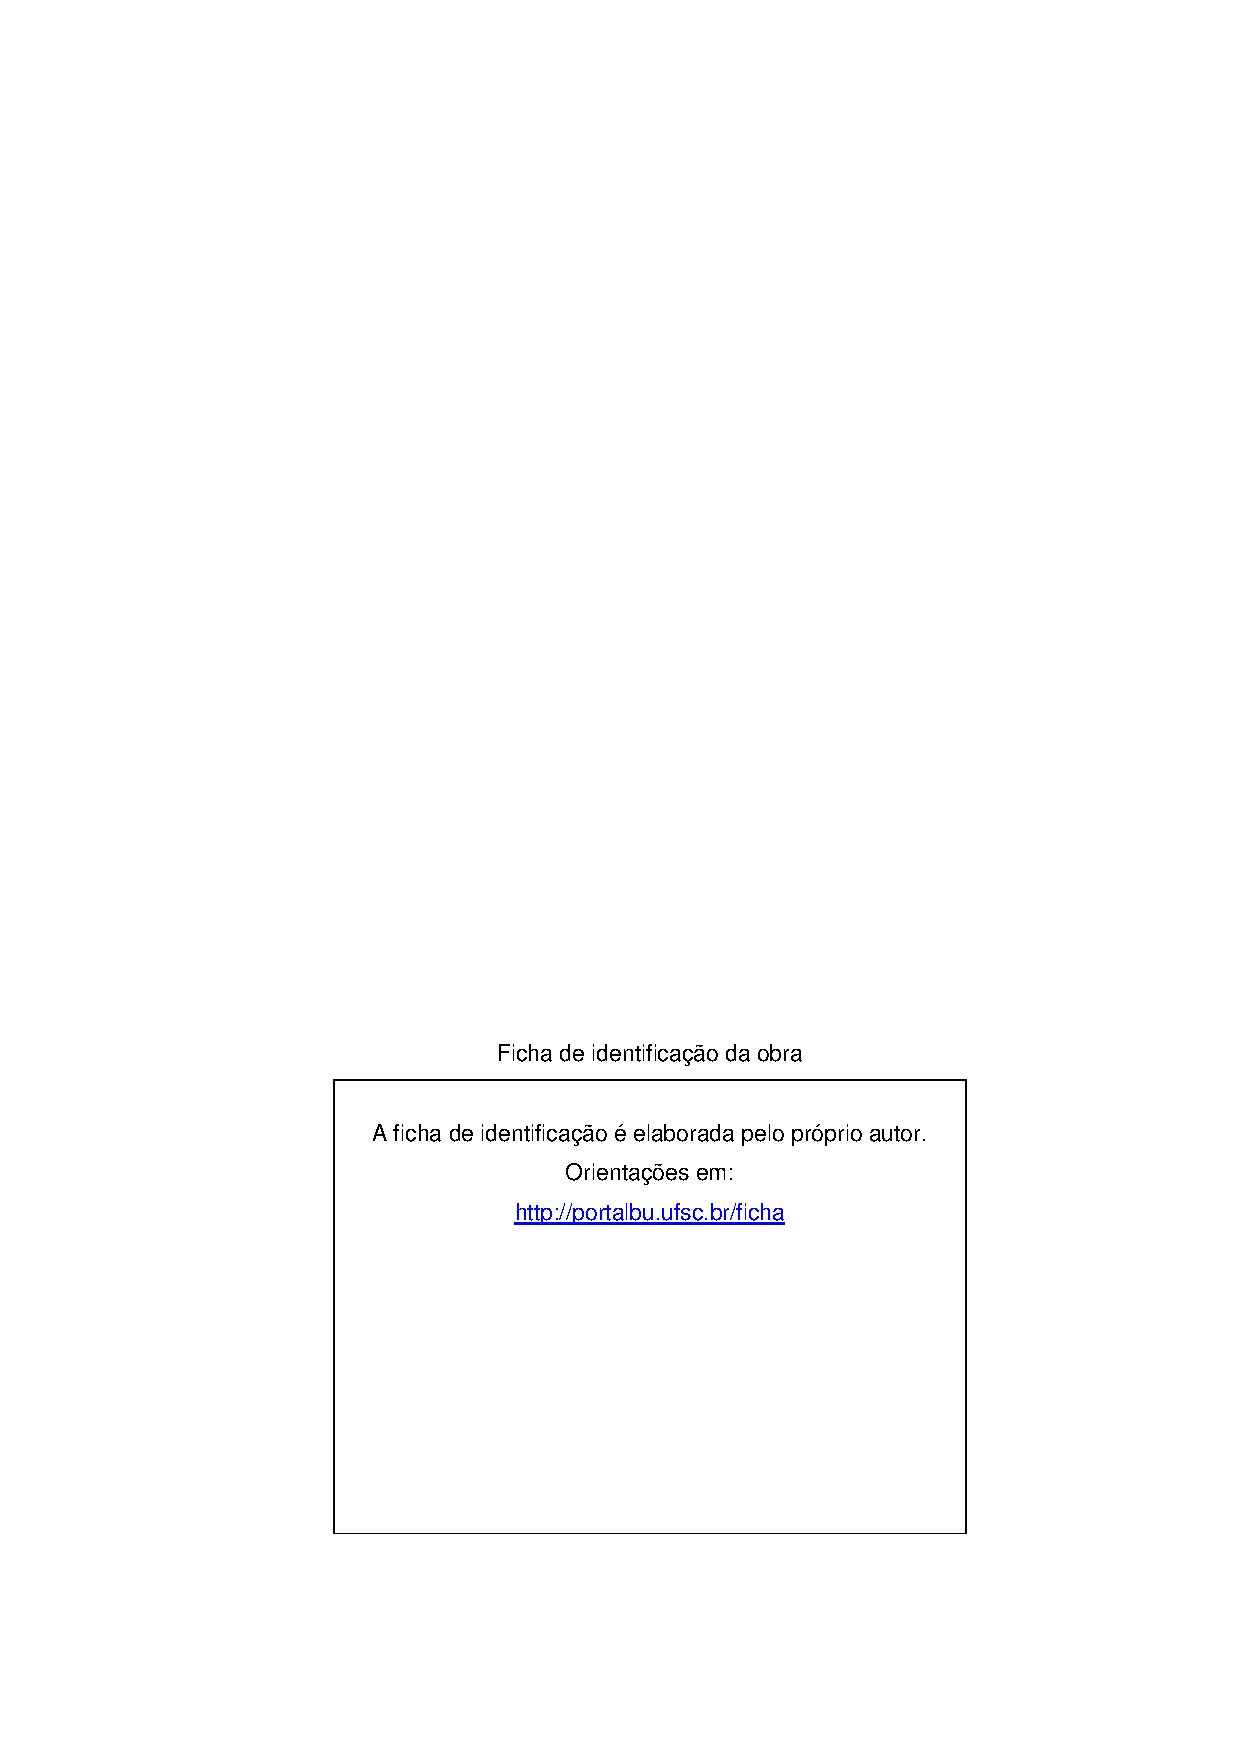
\includepdf{beforetext/Ficha_Catalografica.pdf}
\end{fichacatalografica}
% ---

% ---
% Inserir folha de aprovação
% ---
\begin{folhadeaprovacao}
	\OnehalfSpacing
	\centering
	\imprimirautor\\%
	\vspace*{10pt}		
	\textbf{\imprimirtitulo}%
	\ifnotempty{\imprimirsubtitulo}{:~\imprimirsubtitulo}\\%
	%		\vspace*{31.5pt}%3\baselineskip
	\vspace*{\baselineskip}
	%\begin{minipage}{\textwidth}
	O presente trabalho em nível de \imprimirnivel~foi avaliado e aprovado por banca examinadora composta pelos seguintes membros:\\
	%\end{minipage}%
	\vspace*{\baselineskip}
	Prof. Dr. Odorico Machado Mendizabal \\
	Universidade Federal de Santa Catarina \\
	\vspace*{\baselineskip}
	Prof.(a) xxxx, Dr(a).\\
	Instituição xxxx\\
        \vspace*{\baselineskip}
	Prof.ª Dr.ª Atslands Rego da Rocha \\
	Universidade Federal do Ceará \\
	\vspace*{2\baselineskip}
	\begin{minipage}{\textwidth}
		Certificamos que esta é a \textbf{versão original e final} do trabalho de conclusão que foi julgado adequado para obtenção do título de \imprimirformacao.\\
	\end{minipage}
	%    \vspace{-0.7cm}
	\vspace*{\fill}
	\assinatura{\OnehalfSpacing Coordenação do Programa de Pós-Graduação}
	\vspace*{\fill}
	\assinatura{\OnehalfSpacing\imprimirorientador \\ \imprimirorientadorRotulo}
	%	\ifnotempty{\imprimircoorientador}{
	%	\assinatura{\imprimircoorientador \\ \imprimircoorientadorRotulo \\
	%		\imprimirinstituicao~--~\imprimirinstituicaosigla}
	%	}
	% \newpage
	\vspace*{\fill}
	\imprimirlocal, \imprimirano.
\end{folhadeaprovacao}
% ---

% ---
% Dedicatória
% ---
\begin{dedicatoria}
	\vspace*{\fill}
	\noindent
	\begin{adjustwidth*}{}{5.5cm} 
		\raggedleft       
		Dedico este trabalho a todos os meus professores, 
sendo, meus pais, os maiores entre eles.
	\end{adjustwidth*}
\end{dedicatoria}
% ---

% ---
% Agradecimentos
% ---
\begin{agradecimentos}
    Neste momento, sinto uma gratidão imensa por cada pessoa que fez parte desta jornada. Agradeço de coração aos meus pais e à minha namorada, cujos amores incondicionais e apoios constantes foram a base sólida sobre a qual construí meus sonhos e conquistas. Sem vocês, nada disso teria sido possível.

    À UFSC (Universidade Federal de Santa Catarina) e a todos os seus membros, expresso meu profundo agradecimento. Cada professor, funcionário e colega desempenhou um papel crucial no meu crescimento acadêmico. Através do ensino de qualidade, das valiosas ferramentas e dos recursos disponibilizados, pude adquirir o conhecimento necessário para realizar este trabalho.

    Em especial, minha orientadora Patrícia Della Méa Plentz, você foi uma inspiração e guia ao longo dessa jornada. Sua dedicação, sabedoria e orientação foram fundamentais para a construção desta qualificação. Agradeço por compartilhar seu conhecimento, suas perspectivas e por me motivar a alcançar meu melhor desempenho. Sua generosidade em investir tempo e energia em minha formação é um presente inestimável.

    Um agradecimento especial à LexisNexis, em especial a Mauro Marques e Alysson Oliveira. Sua colaboração e apoio foram cruciais para o desenvolvimento deste trabalho. Suas expertise e capacidade analítica, com seu suporte técnico e encorajamento constante, enriqueceram imensamente minha pesquisa. Sou profundamente grato(a) a ambos por sua dedicação e por acreditarem no potencial deste projeto.


    A todos vocês, meus pais, minha namorada, minha orientadora e a equipe da LexisNexis, sou profundamente grato(a). Seus ensinamentos, apoio e encorajamento foram a força motriz que me impulsionou a superar desafios e alcançar meus objetivos. Cada palavra de incentivo, cada gesto de apoio e cada momento de aprendizado deixaram uma marca indelével em minha vida acadêmica e pessoal.

    Expresso minha sincera admiração e gratidão por cada contribuição que fizeram em minha jornada. Vocês são verdadeiros pilares em minha vida, e sou grato(a) por terem acreditado em mim e por terem compartilhado esse caminho comigo.

\end{agradecimentos}
% ---

% ---
% Epígrafe
% ---
\begin{epigrafe}
	\vspace*{\fill}
	\begin{flushright}
		\textit{''A educação é a arma mais poderosa que \\
            você pode usar para mudar o mundo.'' \\
            (Nelson Mandela)
            }
	\end{flushright}
\end{epigrafe}
% ---

% ---
% RESUMOS
% ---

% resumo em português
\setlength{\absparsep}{18pt} % ajusta o espaçamento dos parágrafos do resumo
\begin{resumo}
	\SingleSpacing
	Este trabalho apresentou o desenvolvimento e a avaliação de uma arquitetura modular para ambientes de computação em névoa, projetada para suportar comunicação direta entre diferentes domínios e integrar dispositivos de borda, nós de névoa e a nuvem, tomando como referência o modelo do OpenFog Consortium. A solução foi construída com base nos pilares de escalabilidade, abertura, autonomia, programabilidade e hierarquia, considerando o contexto de cidades inteligentes. A proposta incorporou abstração de protocolos para permitir interoperabilidade entre diferentes tecnologias de comunicação, além de um mecanismo de balanceamento dinâmico de carga e agregação de dados para otimizar o uso de recursos e reduzir o tráfego de dados para a nuvem. A metodologia envolveu a simulação de dois dias de operação contínua, com dispositivos distribuídos em dois domínios de névoa e geração periódica de dados, analisando métricas de latência, consumo de memória, throughput, taxa de entrega e fator de agregação. Os resultados indicaram latência ponta a ponta média de 15,6 ms, taxa de entrega de 100\% e redução de aproximadamente 99,97\% nas requisições à nuvem, mantendo desempenho compatível com aplicações sensíveis ao tempo. A comparação com trabalhos como o EXEGESIS evidenciou diferenças no gerenciamento de serviços e na flexibilidade de adaptação a novos cenários, destacando vantagens na separação entre a camada de aplicação e a de protocolos. Entre as perspectivas futuras estão a implementação de autenticação e criptografia ponta a ponta, estratégias de recuperação automática e validação da arquitetura em domínios como saúde conectada e transporte inteligente.
	
	\textbf{Palavras-chave}: computação em névoa. interoperabilidade. balanceamento de carga.
\end{resumo}

% resumo em inglês
\begin{resumo}[Abstract]
	\SingleSpacing
	\begin{otherlanguage*}{english}
		This research presented the development and evaluation of a modular architecture for fog computing environments, designed to support direct communication between different domains and to integrate edge devices, fog nodes, and the cloud, taking the OpenFog Consortium reference model as a guideline. The solution was built on the pillars of scalability, openness, autonomy, programmability, and hierarchy, within the context of smart cities. The proposal incorporated protocol abstraction to enable interoperability among different communication technologies, along with a dynamic load balancing mechanism and data aggregation to optimize resource usage and reduce cloud traffic. The methodology involved simulating two days of continuous operation, with devices distributed across two fog domains and generating periodic data, analyzing metrics such as latency, memory consumption, throughput, delivery rate, and aggregation factor. The results indicated an average end-to-end latency of 15.6 ms, a delivery rate of 100\%, and approximately 99.97\% reduction in cloud requests, maintaining performance compatible with time-sensitive applications. Comparison with works such as EXEGESIS highlighted differences in service management and adaptability to new scenarios, with advantages in the separation between the application and protocol layers. Future perspectives include implementing end-to-end authentication and encryption, automatic recovery strategies, and validating the architecture in domains such as connected healthcare and intelligent transportation.

		\textbf{Keywords}: fog computing. interoperability. load balancing.
	\end{otherlanguage*}
\end{resumo}


%% resumo em francês 
%\begin{resumo}[Résumé]
% \begin{otherlanguage*}{french}
%    Il s'agit d'un résumé en français.
% 
%   \textbf{Mots-clés}: latex. abntex. publication de textes.
% \end{otherlanguage*}
%\end{resumo}
%
%% resumo em espanhol
%\begin{resumo}[Resumen]
% \begin{otherlanguage*}{spanish}
%   Este es el resumen en español.
%  
%   \textbf{Palabras clave}: latex. abntex. publicación de textos.
% \end{otherlanguage*}
%\end{resumo}
%% ---

{%hidelinks
	\hypersetup{hidelinks}
	% ---
	% inserir lista de ilustrações
	% ---
	\pdfbookmark[0]{\listfigurename}{lof}
	\listoffigures*
	\cleardoublepage
	% ---
	
	% ---
	% inserir lista de quadros
	% ---
	\pdfbookmark[0]{\listofquadrosname}{loq}
	\listofquadros*
	\cleardoublepage
	% ---
	
	% ---
	% inserir lista de tabelas
	% ---
	\pdfbookmark[0]{\listtablename}{lot}
	\listoftables*
	\cleardoublepage
	% ---
	
	% ---
	% inserir lista de abreviaturas e siglas (devem ser declarados no preambulo)
	% ---
	\imprimirlistadesiglas
	% ---
	
	% ---
	% inserir lista de símbolos (devem ser declarados no preambulo)
	% ---
	\imprimirlistadesimbolos
	% ---
	
	% ---
	% inserir o sumario
	% ---
	\pdfbookmark[0]{\contentsname}{toc}
	\tableofcontents*
	\cleardoublepage
	
}%hidelinks
% ---
% ---

% ----------------------------------------------------------
% ELEMENTOS TEXTUAIS
% ----------------------------------------------------------
\textual

% ---
% 1 - Introdução
% ---
% ----------------------------------------------------------
\chapter{Introdução}\label{cap:introducao}
% ----------------------------------------------------------

Estamos vivenciando um crescimento exponencial no número de dispositivos conectados à internet, impulsionado principalmente pela expansão da Internet das Coisas (IoT). Essa categoria abrange uma ampla gama de equipamentos, como smartphones, relógios inteligentes, sensores ambientais, eletrodomésticos inteligentes e veículos autônomos, entre outros. Esses dispositivos diferem significativamente entre si em termos de capacidade computacional, armazenamento local, autonomia energética e protocolos de comunicação utilizados, o que introduz desafios consideráveis de interoperabilidade e gerenciamento em larga escala.

Paralelamente, cresce a exigência por processamento de dados em tempo quase real, especialmente em aplicações de missão crítica. Veículos autônomos, por exemplo, precisam realizar inferências e tomar decisões instantâneas com base em grandes volumes de dados sensoriais \cite{markakis2017}. Da mesma forma, em cenários de saúde digital, dispositivos vestíveis como \textit{smartwatches} monitoram sinais vitais continuamente e podem enviar alertas automáticos a instituições médicas, possibilitando respostas emergenciais, como o envio imediato de ambulâncias em situações críticas \cite{cassel2024}.

Diante desse cenário, a arquitetura de computação em névoa (\textit{fog computing}) surgiu como uma solução eficaz para suprir a necessidade de processamento e armazenamento mais próximos da borda da rede. Essa abordagem reduz a latência e melhora a eficiência do sistema, sendo especialmente relevante em aplicações que exigem respostas rápidas e precisas. A computação em névoa ainda pode atuar como intermediária entre os dispositivos e a nuvem, realizando um pré-processamento local dos dados antes de enviá-los para a nuvem, o que facilita a integração, reduz o tráfego e diminui a carga sobre os servidores centrais.

Na Figura~\ref{fig:arquitetura_basica}, temos ilustrado uma arquitetura básica de névoa, os dispositivos enviam dados para os equipamentos da camada de névoa, onde ocorre o processamento local. Os dados processados podem então ser devolvidos para os dispositivos ou encaminhados à nuvem, dependendo do contexto da aplicação.

\begin{figure}[htb]
	\caption{\label{fig:arquitetura_basica}Arquitetura básica de comunicação na computação em névoa.}
	\begin{center}
		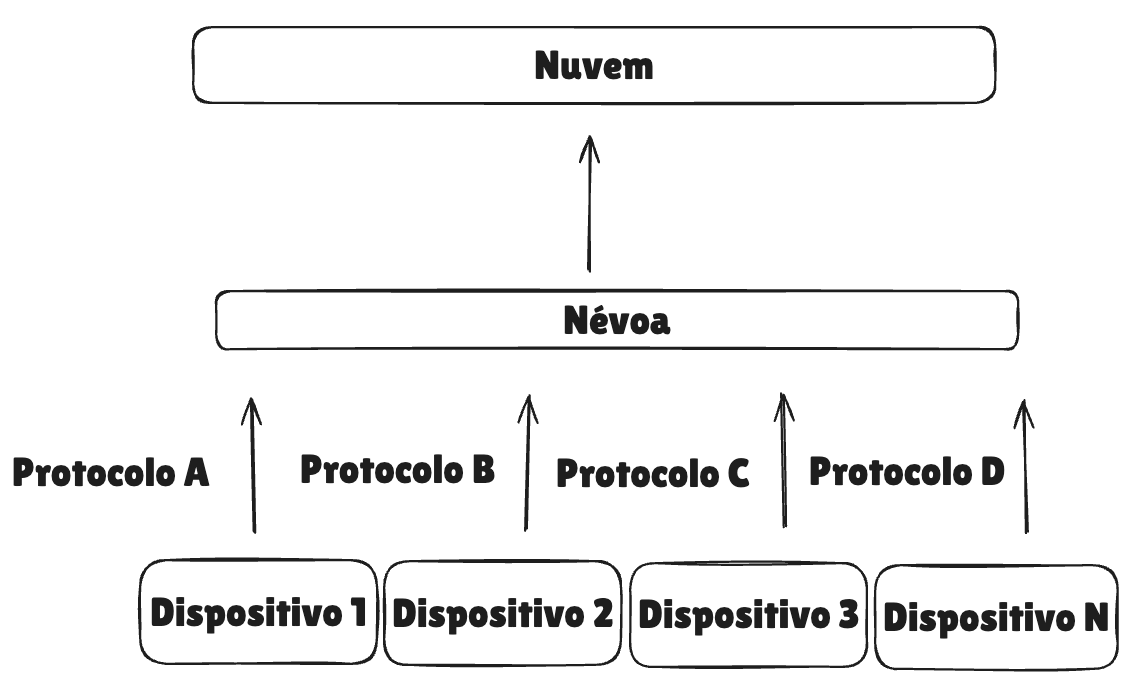
\includegraphics[width=0.7\linewidth]{images/arquitetura_basica.png}
	\end{center}
	\fonte{Do autor.}
\end{figure}

No entanto, a diversidade de dispositivos e protocolos de comunicação ainda representa um obstáculo à interoperabilidade plena. A ausência de um padrão universalmente aceito dificulta a comunicação eficiente entre equipamentos heterogêneos.

Para abordar esses desafios, este trabalho propõe uma arquitetura de névoa modular com suporte à comunicação entre diferentes névoas, a qual é composta por três camadas principais, descritas a seguir:

\begin{itemize}
    \item \textbf{Nó de Névoa Primário:} responsável por atuar como ponto de entrada da arquitetura de névoa. Ele realiza a conversão de protocolos de comunicação, o balanceamento de carga entre os demais nós de névoa e outros nós primários, além de localizar e coordenar os nós de névoa disponíveis.

    \item \textbf{Nó de Névoa:} recebe os dados encaminhados pelo nó primário, realiza o pré-processamento local conforme a lógica da aplicação, e transmite os resultados ao nó agregador.

    \item \textbf{Nó Agregador:} responsável por consolidar os dados processados pelos diversos nós de névoa em um único arquivo ou estrutura de dados, facilitando sua transmissão para a nuvem.
\end{itemize}

% ----------------------------------------------------------
\section{Objetivos}
% ----------------------------------------------------------

Nas seções abaixo estão descritos o objetivo geral e os objetivos 
específicos.

% ----------------------------------------------------------
\subsection{Objetivo Geral}
% ----------------------------------------------------------

Desenvolver uma arquitetura modular de computação em névoa voltada à comunicação entre diferentes névoas, com foco na integração de novos dispositivos, e na facilitação da interoperabilidade entre protocolos distintos, considerando aplicações cujos requisitos possam ser contemplados por essa abordagem.

% ----------------------------------------------------------
\subsection{Objetivos Específicos}
% ----------------------------------------------------------

Para atender ao objetivo geral descrito nesta seção, apresentam-se os seguintes objetivos específicos:

\begin{itemize}
  \item Desenvolver uma arquitetura modular em camadas para a computação em névoa, definindo as funções e responsabilidades de cada camada, com foco na integração de novos dispositivos.
  
  \item Projetar e implementar um sistema de comunicação entre névoas, visando facilitar a interoperabilidade e reduzir a latência entre dispositivos que utilizam diferentes padrões e tecnologias, atendendo a aplicações cujos requisitos sejam compatíveis com a arquitetura.

  \item Desenvolver e integrar mecanismos de conversão de protocolos, permitindo a comunicação entre dispositivos com diferentes padrões e tecnologias.

  \item Avaliar a eficácia da arquitetura modular proposta por meio da medição de tempo de resposta, latência e quantidade de pacotes com e sem falhas, em simulações que reproduzam requisitos específicos das aplicações.

  \item Documentar os resultados obtidos e propor diretrizes, fornecendo orientações e melhores práticas para futuras implementações e pesquisas que atendam a requisitos similares.
\end{itemize}

% ---

% ---
% 2 - Fundamentação Teórica
% ---
% ----------------------------------------------------------
\chapter{Fundamentação Teórica}
% ----------------------------------------------------------

Primeiramente, para que se possa compreender o contexto deste trabalho, é necessária a revisão de alguns conceitos fundamentais. Desta forma, iniciamos com a conceituação do que é computação distribuída e em névoa e avançamos nos conceitos pertinentes a este trabalho.

% ----------------------------------------------------------
\section{Computação em Nuvem}
% ----------------------------------------------------------

A computação em nuvem é uma tecnologia que permite o acesso remoto a recursos computacionais, como servidores, armazenamento de dados, redes e software, através da internet. Essa abordagem oferece uma maneira eficiente de fornecer serviços de TI sob demanda, proporcionando flexibilidade, escalabilidade e redução de custos. A computação em nuvem envolve a utilização de data centers distribuídos para fornecer esses recursos, permitindo que os usuários acessem e utilizem capacidades computacionais de acordo com suas necessidades, sem a necessidade de investir em hardware próprio \cite{tanenbaum2015}.

Os modelos de serviço da computação em nuvem são geralmente classificados em três categorias principais: Infraestrutura como Serviço (IaaS), Plataforma como Serviço (PaaS) e Software como Serviço (SaaS). No modelo IaaS, os provedores de nuvem oferecem recursos virtualizados, como servidores e armazenamento, que os clientes podem configurar e gerenciar conforme suas necessidades. Esse modelo é ideal para empresas que necessitam de controle sobre a infraestrutura e desejam a flexibilidade de escalar seus recursos conforme a demanda. Exemplos de IaaS incluem Amazon Web Services (AWS) e Microsoft Azure.

No modelo PaaS, a nuvem fornece uma plataforma que permite aos desenvolvedores criar, testar e implantar aplicações sem se preocupar com a gestão da infraestrutura subjacente. Tanenbaum e Bos destacam que o PaaS simplifica o processo de desenvolvimento ao fornecer um ambiente integrado com ferramentas e serviços necessários para a construção de aplicações. Exemplos de PaaS incluem Google App Engine e Heroku.

O modelo SaaS oferece aplicações de software através da internet, eliminando a necessidade de instalação e manutenção de software localmente nos dispositivos dos usuários. As aplicações SaaS são acessíveis via navegador web, proporcionando uma experiência de uso simplificada e atualizações automáticas. Exemplos populares de SaaS incluem Google Workspace, Microsoft Office 365 e Salesforce.

Tanenbaum e Bos enfatizam que a computação em nuvem também proporciona vantagens significativas em termos de continuidade de negócios e recuperação de desastres. Ao armazenar dados e executar aplicações em data centers distribuídos geograficamente, a nuvem garante que as operações possam ser retomadas rapidamente em caso de falhas locais, aumentando a resiliência e a segurança das operações.

% ----------------------------------------------------------
\section{Computação em Névoa}
% ----------------------------------------------------------

A computação em névoa, também conhecida como fog computing, surge como uma extensão do paradigma de computação em nuvem, oferecendo uma solução para as limitações de latência e largura de banda enfrentadas na nuvem centralizada. Diferente da computação em nuvem, onde os dados são processados em data centers distantes, a computação em névoa distribui recursos computacionais, de armazenamento e serviços ao longo da borda da rede, mais próximos dos dispositivos finais. Esta abordagem hierárquica envolve dispositivos finais, nós de névoa e a nuvem centralizada, permitindo a distribuição eficiente de tarefas e o processamento local de dados, essencial para aplicações que exigem alta responsividade e baixa latência \cite{rahmani2018}.

Entre as principais vantagens da computação em névoa, destaca-se a redução significativa da latência, crucial para aplicações em tempo real, como veículos autônomos e sistemas de saúde conectados. Além disso, a economia de largura de banda é alcançada através do pré-processamento e filtragem de dados localmente, diminuindo a quantidade de dados transmitidos para a nuvem. A segurança e privacidade dos dados são aprimoradas ao processar informações sensíveis localmente, reduzindo os riscos durante a transmissão. A alta disponibilidade e resiliência dos serviços também são beneficiadas pela distribuição de recursos em múltiplos nós de névoa, aumentando a robustez do sistema contra falhas.

No contexto da Internet das Coisas (IoT), a computação em névoa revela-se particularmente relevante, suportando aplicações como cidades inteligentes, saúde conectada e a Indústria 4.0. Em cidades inteligentes, a névoa possibilita o monitoramento e controle eficientes de tráfego, energia e segurança pública. Na área da saúde, permite o monitoramento remoto de pacientes e análise de dados médicos em tempo real. Na indústria, a névoa facilita a automação, manutenção preditiva e otimização de processos, promovendo a eficiência operacional e a inovação. Esses exemplos demonstram como a computação em névoa pode transformar diversos setores, proporcionando benefícios significativos em termos de desempenho e confiabilidade.

Apesar das vantagens, a computação em névoa enfrenta desafios como a heterogeneidade dos dispositivos, a complexidade na gestão de recursos distribuídos e a necessidade de padrões interoperáveis.

% ----------------------------------------------------------
\section{Protocolos}
% ----------------------------------------------------------

Os protocolos de comunicação são fundamentais para o funcionamento das redes de computadores e para a troca eficiente e segura de informações entre dispositivos. Eles definem um conjunto de regras e normas que permitem a comunicação entre diferentes sistemas, sejam eles locais ou distribuídos globalmente \cite{tanenbaum2011}. Na computação em névoa, os protocolos são usados para garantir a comunicação eficiente e segura entre dispositivos e servidores locais, permitindo a troca de informações de forma robusta e confiável.

HTTP (Hypertext Transfer Protocol) é um protocolo de requisição-resposta usado principalmente para a troca de informações na web. Ele opera sobre a camada de transporte TCP/IP e permite a comunicação entre clientes (navegadores web) e servidores. Os métodos mais comuns incluem GET (para recuperar dados) e POST (para enviar dados). O HTTP é sem estado, o que significa que cada requisição é independente, simplificando o design do servidor, mas pode necessitar de gerenciamento adicional para manter sessões de usuário \cite{gourley2002}.

WebSocket é um protocolo de comunicação que proporciona um canal bidirecional e full-duplex sobre uma única conexão TCP. Diferente do HTTP, que segue um modelo de requisição-resposta, o WebSocket permite que dados sejam enviados e recebidos de ambos os lados a qualquer momento após a conexão inicial. Isso o torna ideal para aplicações que necessitam de atualizações em tempo real, como chats, jogos online e sistemas de trading financeiro, oferecendo menor latência e maior eficiência \cite{wang2013}.

SFTP (Secure File Transfer Protocol) é um protocolo para transferência segura de arquivos que utiliza criptografia SSH para proteger a confidencialidade e integridade dos dados durante a transferência. Diferente do FTP tradicional, que transmite dados em texto claro, o SFTP encripta tanto os comandos quanto os dados, proporcionando uma camada adicional de segurança. É amplamente utilizado em ambientes que requerem troca segura de arquivos, como empresas e instituições acadêmicas, onde a proteção dos dados é crucial \cite{barrett2005}.

CoAP (Constrained Application Protocol) é um protocolo projetado para dispositivos restritos e redes de baixa capacidade, típico no contexto da Internet das Coisas (IoT). Baseado no modelo de requisição-resposta do HTTP, CoAP é otimizado para operar sobre UDP, resultando em menor sobrecarga de comunicação e melhor desempenho em redes de baixa capacidade. CoAP suporta mecanismos de confiabilidade e é interoperável com HTTP, facilitando a integração entre dispositivos IoT e a web tradicional \cite{bormann2012}.

% ----------------------------------------------------------
\section{GraphQL}
% ----------------------------------------------------------

GraphQL é uma linguagem de consulta e manipulação de dados para APIs que foi desenvolvida pelo Facebook em 2012 e lançada como um projeto de código aberto em 2015. Em contraste com o tradicional modelo REST (Representational State Transfer), GraphQL permite que os clientes solicitem exatamente os dados de que precisam, sem a necessidade de receber informações excedentes. Essa capacidade de seleção pode reduzir o volume de dados transferidos pela rede, resultando em uma maior eficiência tanto na comunicação quanto no desempenho geral das aplicações \cite{silveira2019}.

Uma das principais vantagens do GraphQL é sua flexibilidade na recuperação de dados. Enquanto a arquitetura REST requer múltiplas requisições para diferentes endpoints para compilar dados relacionados, o GraphQL permite que todas essas informações sejam obtidas através de uma única consulta. Isso é possível porque o cliente especifica exatamente quais campos e relacionamentos deseja recuperar, e o servidor responde com os dados estruturados conforme solicitado. Esse modelo de consulta única não apenas simplifica o processo de desenvolvimento, mas também minimiza o tempo de resposta e a carga na rede.

Além disso, o GraphQL facilita a evolução das APIs. No modelo REST, a adição de novos campos ou a alteração da estrutura de dados pode exigir a criação de novas versões de endpoints para garantir a compatibilidade retroativa. Com GraphQL, as APIs podem evoluir de maneira mais fluida. Novos campos podem ser adicionados às respostas sem impactar os clientes existentes, pois cada cliente continua a solicitar apenas os dados específicos de que precisa.

Adicionalmente, a abordagem de GraphQL também melhora a experiência de desenvolvimento ao fornecer uma documentação mais clara e precisa. A própria estrutura da linguagem e as ferramentas associadas, como o GraphiQL, permitem que os desenvolvedores explorem e testem as APIs de maneira interativa. Isso contrasta com a documentação tradicional de APIs REST, que pode ser menos intuitiva e exigir mais esforço para ser mantida e compreendida.

% ----------------------------------------------------------
\section{HPCC Systems}
% ----------------------------------------------------------

O HPCC Systems (\textit{High Performance Computing Cluster}) é uma plataforma de processamento massivamente paralelo, de código aberto, desenvolvida pela divisão HPCC Systems da LexisNexis Risk Solutions. Seu objetivo é lidar com grandes volumes de dados, desde a ingestão até a entrega de produtos de dados, com tempos de resposta reduzidos. Criado antes da popularização do Hadoop, não se baseia no paradigma \textit{map-reduce}, possuindo uma arquitetura própria \cite{taylor2022}.

A plataforma é composta por diversos servidores de infraestrutura responsáveis por funções como compilação de código, gerenciamento distribuído de dados e execução de trabalhos (\textit{workunits}). O processamento é realizado por dois tipos de clusters: Thor e ROXIE.

O Thor é voltado para operações intensivas em grandes conjuntos de dados, realizando tarefas como transformação, limpeza, integração e análise em larga escala. É utilizado como ferramenta de \textit{back office}, transformando dados brutos em produtos finais e executando análises complexas.

O ROXIE (\textit{Rapid Online Xml Inquiry Engine}) é destinado a consultas rápidas e atendimento a solicitações de usuários finais, buscando oferecer respostas em tempos muito reduzidos, frequentemente inferiores a um segundo. É, portanto, o componente voltado ao acesso e entrega de dados processados.

Ambos os clusters utilizam a linguagem ECL (\textit{Enterprise Control Language}), de natureza declarativa. Nessa abordagem, o programador especifica o que deve ser feito, enquanto o sistema determina a forma mais eficiente de execução. Isso contribui para simplificar o desenvolvimento e reduzir a possibilidade de erros.

A arquitetura do HPCC Systems foi concebida para permitir escalabilidade progressiva e operação integrada, incorporando desde a ingestão e transformação de dados até a disponibilização dos resultados, sem depender de ferramentas externas para compor o ambiente de produção. Por ser de código aberto, pode ser implantado tanto em ambientes físicos com hardware convencional quanto em configurações baseadas em contêineres, adaptando-se às necessidades de diferentes cenários de processamento de dados.

% ---

% ---
% 3 - Revisão Bibliográfica
% ---
% ----------------------------------------------------------
\chapter{Revisão Bibliográfica}\label{cap:revisao_bibliografica}
% ----------------------------------------------------------

Para esse trabalho, foram realizadas pesquisas nas bases de dados de artigos científicos, utilizando as seguintes palavras-chaves: 'fog', 'fog' AND 'architecture', e aplicado um filtro para os últimos 5 anos, ou seja, de 2020 até 2024, e obtivemos a quantidade de artigos que podemos visualizar na Tabela~\ref{tab:Tab_ArtigosFog}.

\begin{table}[htb]
	\ABNTEXfontereduzida
	\caption{\label{tab:Tab_ArtigosFog}Quantidade de artigos por palavra-chave e base de dados}
	\begin{tabular}{@{}p{6.5cm}p{3.5cm}p{4cm}@{}}
		\toprule
		\textbf{Palavra-chave} & \textbf{Banco de Dados} & \textbf{Quantidade de Artigos} \\ \midrule
		\multirow[c]{2}{*}{\textbf{\textit{'fog'}}} 
		    & Scopus & 18.970 \\
		    & IEEE   & 6.925  \\ \midrule
		\multirow[c]{2}{*}{\textbf{\textit{'fog' AND 'architecture'}}} 
		    & Scopus & 3.144 \\
		    & IEEE   & 1.749 \\ \midrule
	\end{tabular}
	\fonte{Do autor.}
\end{table}

Com base nos dados da tabela fornecida, observamos que o Scopus lidera com a maior coleção de artigos indexados. Em contraste, o IEEE apresenta uma quantidade relativamente menor.

% ----------------------------------------------------------
\section{Trabalhos Correlatos}\label{cap:trabalhos_relacionados}
% ----------------------------------------------------------

Foram lidos títulos e resumo de 125 artigos, dos quais 25 foram lidos completamente, e desses foram selecionados 5 que apresentam propostas semelhantes à proposta deste trabalho e por isso serão detalhados nas subseções seguintes.

% ----------------------------------------------------------
\subsection{Inter-container Communication Aware Container Placement in Fog Computing}
% ----------------------------------------------------------

Neste trabalho, os autores propõem um algoritmo genético para a colocação de contêineres, destacando a abordagem via RDMA (Remote Direct Memory Access) por sua capacidade de reduzir significativamente a latência de rede e a utilização da CPU do host. O RDMA permite acesso direto à memória de outro host sem envolvimento do sistema operacional, resultando em uma comunicação mais rápida e eficiente. Comparado com os modos Host e Overlay, a comunicação RDMA oferece vantagens significativas em termos de desempenho e redução de latência. Além disso, o artigo aborda a importância do isolamento adequado entre contêineres para garantir a estabilidade e segurança do sistema, aspectos críticos em ambientes de computação em névoa onde múltiplos contêineres compartilham os mesmos recursos físicos.

Os resultados das simulações mostram que a inclusão de RDMA pode melhorar substancialmente o desempenho das aplicações, destacando a importância de selecionar a tecnologia de comunicação inter-contêiner mais adequada para cada situação. Cada contêiner pode utilizar o protocolo de comunicação que melhor se adapta às suas necessidades específicas, proporcionando maior eficiência e flexibilidade na comunicação entre contêineres. Isso permite que os sistemas de computação em névoa mantenham a eficiência e a performance ao lidar com a comunicação entre diversos protocolos, assegurando que cada contêiner opere com o protocolo mais apropriado para suas funções.

% ----------------------------------------------------------
\subsection{EXEGESIS: Extreme Edge Resource Harvesting for a Virtualized Fog Environment}
% ----------------------------------------------------------

Neste trabalho, os autores propõem a arquitetura EXEGESIS, que aborda os desafios de comunicação e processamento de dados na névoa. A arquitetura de três camadas inclui a camada "mist", composta por dispositivos interconectados que formam vizinhanças locais; a camada "vFog", que permite interconexões dinâmicas entre essas vizinhanças; e a camada de nuvem, que oferece recursos abundantes e facilita a interconexão dos elementos vFog. Esta estrutura modular e hierárquica visa melhorar a utilização de recursos, reduzir a latência e melhorar a eficiência do sistema, permitindo a conversão e integração de protocolos diversos.

No contexto da comunicação com diversos protocolos, EXEGESIS propõe uma plataforma de orquestração que facilita a interoperabilidade entre dispositivos utilizando diferentes padrões e tecnologias. A camada "vFog" age como um intermediário virtual, coordenando os recursos e a comunicação entre as névoas e a nuvem, garantindo que dados críticos sejam processados e armazenados onde podem agregar mais valor.

% ----------------------------------------------------------
\subsection{Extending Scalability of IoT/M2M Platforms with Fog Computing}
% ----------------------------------------------------------

Neste trabalho, os autores propõem a migração do oneM2M, uma plataforma global de IoT/M2M, para uma arquitetura de névoa baseada em contêineres hierárquicos. Esta abordagem visa resolver os problemas de escalabilidade e latência ao trazer a capacidade de processamento e armazenamento para mais perto dos dispositivos finais.

Para garantir a comunicação eficiente entre os diversos componentes da arquitetura, o oneM2M suporta a ligação de suas interfaces de comunicação aos protocolos HTTP e CoAP, fornecendo APIs Restful sobre todas essas interfaces. Isso permite que diferentes tipos de dispositivos e serviços se comuniquem de maneira eficaz, utilizando o protocolo mais adequado para cada caso. Por exemplo, HTTP pode ser usado para comunicação de dados mais robusta e complexa, enquanto o CoAP é ideal para dispositivos com restrições de recursos e necessidade de comunicação leve.

% ----------------------------------------------------------
\subsection{Privacy preserving data aggregation with fault tolerance in fog-enabled smart grids}
% ----------------------------------------------------------

Neste trabalho, os autores propõem um esquema de agregação de dados seguro e tolerante a falhas para grades inteligentes (SG) habilitadas por computação em névoa. O estudo aborda os desafios de privacidade e segurança em SG, onde os medidores inteligentes (SM) coletam dados de consumo de eletricidade dos usuários e os transmitem para os provedores. Para garantir a privacidade, o esquema utiliza o criptossistema Boneh-Goh-Nissam (BGN) para criptografar os dados de medição e o algoritmo de assinatura digital de curva elíptica (ECDSA) para autenticação da fonte. A tolerância a falhas é assegurada ao permitir que os nós de névoa (FN) substituam os dados dos medidores com falha pelos últimos dados válidos armazenados, sem a necessidade de comunicação adicional com autoridades confiáveis.

O estudo também destaca a importância de proteger os dados dos consumidores em grades inteligentes, onde a agregação segura de dados é crucial para evitar a divulgação de informações sensíveis. A arquitetura baseada em névoa permite a agregação de dados próximo aos usuários finais, reduzindo a latência e os custos de comunicação. A utilização de criptografia homomórfica permite operações sobre dados criptografados, mantendo a privacidade dos usuários. A abordagem adotada assegura que, mesmo em presença de medidores defeituosos, a agregação de dados continua eficaz e eficiente, fornecendo resultados estimativos precisos para a gestão de eletricidade nas grades inteligentes.

% ----------------------------------------------------------
\subsection{FPDA: Fault-Tolerant and Privacy-Enhanced Data Aggregation Scheme in Fog-Assisted Smart Grid}
% ----------------------------------------------------------

Neste trabalho, os autores propõem a agregação de dados em redes inteligentes (SG) com foco na preservação da privacidade e tolerância a falhas. O FPDA propõe um método de agregação de dados que permite a disponibilidade de dados e a preservação da privacidade simultaneamente. A tolerância a falhas garante que a descriptografia possa ser realizada com sucesso mesmo que alguns medidores inteligentes (SMs) falhem, sem a necessidade de uma autoridade confiável centralizada ou atualizações de chaves após cada recuperação de falha.

A abordagem FPDA utiliza uma criptografia homomórfica aditiva, onde a descriptografia do texto cifrado agregado é equivalente à soma direta de todas as leituras em texto claro. O esquema é projetado para operar eficientemente em uma arquitetura assistida por névoa (fog), onde os nós de névoa (FNs) realizam a agregação de dados antes de transmiti-los ao centro de controle (CC). Quando alguns SMs falham, os FNs iniciam interações adicionais de solicitação-resposta com um número limitado de SMs para reconstruir as chaves parciais necessárias. Esse método, baseado em um esquema de compartilhamento de segredo de limite (tSSS) estendido, permite que os SMs reconstruam segredos subsequentes sem revelar suas ações originais, mantendo assim a privacidade e a segurança.

% ----------------------------------------------------------
\section{Comparativo com Trabalhos Correlatos}
% ----------------------------------------------------------

A tabela 2 apresenta um comparativo entre as propostas apresentadas na literatura e a proposta deste trabalho, destacando as características atendidas por cada uma. A proposta deste trabalho se diferencia das demais por algumas razões. Primeiramente, a arquitetura modular proposta para cada nó da névoa inclui múltiplas camadas, cada uma com funções específicas que facilitam a manutenção e a flexibilidade do sistema. Isso contrasta com outras propostas que geralmente utilizam uma aplicação monolítica ou o uso de containers. A abordagem monolítica, embora simplificada em termos de implantação inicial, apresenta desafios em termos de manutenção e escalabilidade. Já o uso de containers, apesar de proporcionar uma certa modularidade, pode enfrentar problemas relacionados ao empacotamento e à sobrecarga de gerenciamento de múltiplos containers.

\begin{table}[htb]
	\ABNTEXfontereduzida
	\caption{\label{tab:Tab_ComparativoPorCaracteristica}Características atendidas por proposta}
	\begin{tabular}{@{}p{6.5cm}p{7.5cm}@{}}
		\toprule
		\textbf{Característica} & \textbf{Propostas que atendem} \\ \midrule
		Uso de RDMA                     & Proposta 1 \\ \midrule
		Uso de Contêineres             & Proposta 1; Proposta 2; Proposta 3 \\ \midrule
		Arquitetura Modular            & Este Trabalho \\ \midrule
		Suporte a Múltiplos Protocolos & Proposta 1; Proposta 2; Proposta 3; Este Trabalho \\ \midrule
		Camada de Serviço Flexível     & Este Trabalho \\ \midrule
		Comunicação entre Névoas       & Este Trabalho \\ \midrule
		Criptografia Homomórfica       & Proposta 4 \\ \midrule
		A aplicação no nó é monolítica & Proposta 4; Proposta 5 \\ \bottomrule
	\end{tabular}
	\fonte{Do autor.}
\end{table}

Na arquitetura proposta nesse trabalho, o fluxo de dados inicia na borda, onde o nó primário da névoa atua como ponto de entrada, registrando os medidores conectados, realizando o balanceamento de carga e, quando necessário, redirecionando solicitações excedentes para outros domínios de névoa que disponham de maior capacidade de processamento.

Cada nó da névoa é estruturado em três camadas. A camada de protocolos é responsável por receber e transmitir dados em diferentes formatos. A camada de processamento gerencia os elementos essenciais para a operação do nó, realizando armazenamento temporário e interações internas necessárias para manter o funcionamento contínuo. Já a camada de serviço executa aplicações configuráveis que processam os dados conforme a lógica da aplicação, preparando-os para as próximas etapas.

Após o processamento nos nós especializados, as informações seguem para um nó agregador, que consolida dados provenientes de múltiplas névoas em arquivos estruturados, otimizando o tráfego antes do envio à nuvem e preparando o material para análises em larga escala.

Conforme apresentado anteriormente, essa proposta apresenta alguns diferenciais em relação aos trabalhos correlatos. A arquitetura proposta para a comunicação entre névoas será explicada em detalhes a seguir.

% ---

% ---
% 4 - Proposta
% ---
% ----------------------------------------------------------
\chapter{Proposta}\label{cap:proposta}
% ----------------------------------------------------------

Este capítulo descreve a arquitetura modular de computação em névoa desenvolvida ao longo deste trabalho. O conteúdo está organizado para apresentar, inicialmente, a visão geral e o papel de cada tipo de nó. Em seguida, são detalhados os componentes, a organização interna dos nós de névoa, os mecanismos de comunicação entre domínios e o fluxo de dados previsto no sistema.

% ----------------------------------------------------------
\section{Visão Geral}
% ----------------------------------------------------------

A arquitetura proposta é composta por três tipos de nós, cada um com responsabilidades distintas no fluxo de dados e na coordenação do processamento distribuído. O nó primário atua como ponto de entrada de um domínio de névoa, gerenciando dispositivos, distribuindo carga e coordenando a comunicação com outros domínios. Os nós de névoa executam o processamento local e oferecem serviços configuráveis para tratamento dos dados. O nó agregador consolida e organiza as informações processadas antes do envio à nuvem.

A Figura~\ref{fig:arquitetura_proposta} apresenta uma visão de alto nível, mostrando o caminho percorrido pelos dados desde os dispositivos na borda até a nuvem, incluindo as interações e responsabilidades de cada tipo de nó.

\begin{figure}[htb]
    \caption{\label{fig:arquitetura_proposta}Visão geral da arquitetura proposta.}
    \begin{center}
        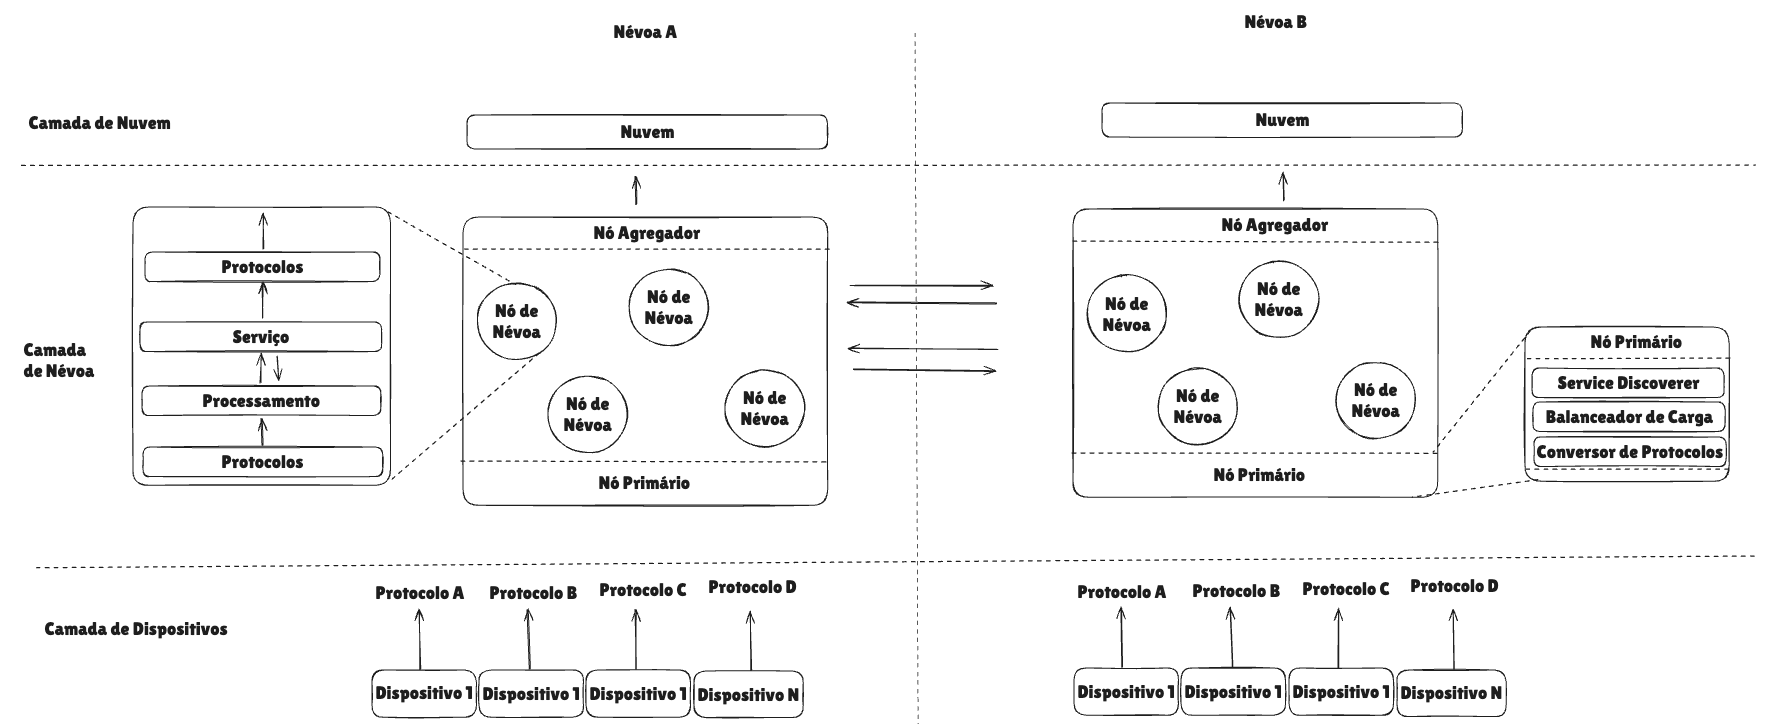
\includegraphics[width=1\linewidth]{images/arquitetura_proposta.png}
    \end{center}
    \fonte{Do autor.}
\end{figure}

% ----------------------------------------------------------
\section{Componentes}
% ----------------------------------------------------------

Esta seção apresenta, em detalhe, as funções e responsabilidades de cada tipo de nó que compõe a arquitetura: nó primário, nós de névoa e nó agregador.

% ----------------------------------------------------------
\subsection{Nó Primário}
% ----------------------------------------------------------

O nó primário funciona como o ponto inicial de contato para dispositivos e novos nós que ingressam em uma névoa. Assim que um nó de névoa é iniciado, ele envia ao nó primário um conjunto de atributos que descrevem sua capacidade, especializações e estado atual de operação. Essas informações são registradas e mantidas para permitir a localização de recursos disponíveis na própria névoa.

Ao receber uma requisição, o nó primário identifica os atributos necessários para o processamento e verifica, entre os nós registrados, quais correspondem ao perfil solicitado. O balanceamento entre os nós locais segue um padrão que procura alternar os destinos de forma equilibrada, em comportamento semelhante a um esquema round robin, sempre respeitando as características solicitadas por cada carga.

Se a análise indicar que não haverá nós suficientes na névoa local para atender à demanda, o nó primário envia uma solicitação para que todos os nós primários de outras névoas informem o estado atual de seus recursos. Esse processo lembra o funcionamento de um protocolo de fofoca, mas é otimizado para reduzir o tráfego de rede, mantendo apenas as trocas essenciais. Com base nas respostas, é selecionada uma névoa remota com disponibilidade, e a requisição é encaminhada para processamento.

O nó primário também é capaz de lidar com diferentes tipos de protocolos, incluindo aqueles que exigem atuação como intermediário na comunicação. Em todos os casos, realiza a adequação inicial do canal recebido, interpretando o conteúdo e convertendo-o para um formato interno uniforme antes de encaminhar para um nó local ou remoto.

% ----------------------------------------------------------
\subsection{Nós de Névoa}
% ----------------------------------------------------------

Os nós de névoa realizam o processamento distribuído e foram organizados em uma estrutura interna baseada em camadas, de forma a facilitar a manutenção e permitir a adição de novas funções sem comprometer o restante do sistema.

A primeira camada, denominada protocolos, é responsável por receber as requisições provenientes do nó primário, realizar as verificações e validações necessárias e repassar as informações para a camada seguinte. Essa estrutura é ilustrada na Figura~\ref{fig:camada_protocolos}, onde diferentes servidores de protocolos alimentam um protocolo padrão utilizado internamente.

\begin{figure}[htb]
    \caption{\label{fig:camada_protocolos}Camada de protocolos de um nó de névoa.}
    \begin{center}
        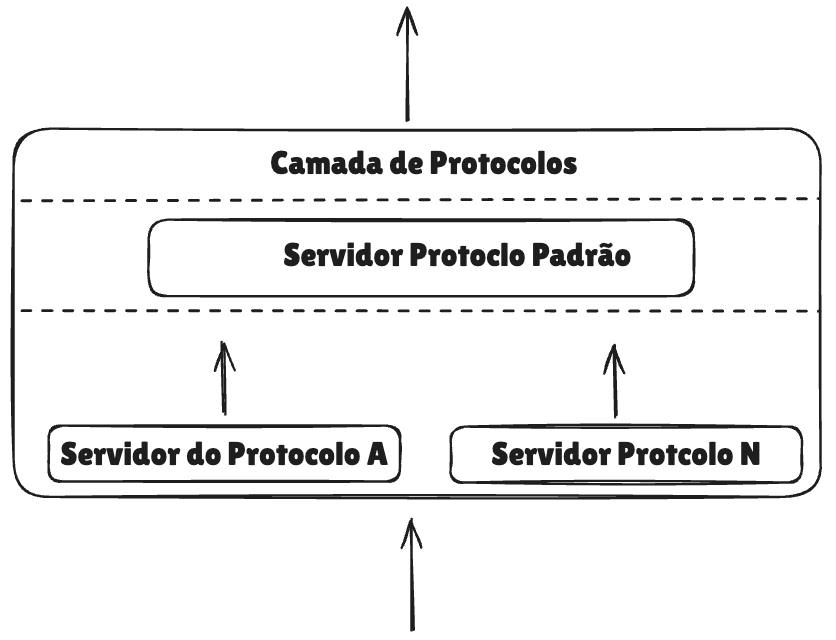
\includegraphics[width=0.7\linewidth]{images/camada_protocolos.png}
    \end{center}
    \fonte{Do autor.}
\end{figure}

A camada de processamento atua como núcleo de coordenação interna, gerenciando a comunicação entre as demais camadas e executando as necessidades específicas do nó de névoa. Essa camada também mantém um mecanismo para consultas internas de dados, permitindo que a camada de serviços acesse apenas as informações estritamente necessárias para seu funcionamento. Além disso, é por meio da camada de processamento que o nó de névoa realiza interações administrativas, como o registro inicial no nó primário. A Figura~\ref{fig:camada_processamento} mostra os principais componentes dessa camada.

\begin{figure}[htb]
    \caption{\label{fig:camada_processamento}Camada de processamento de um nó de névoa.}
    \begin{center}
        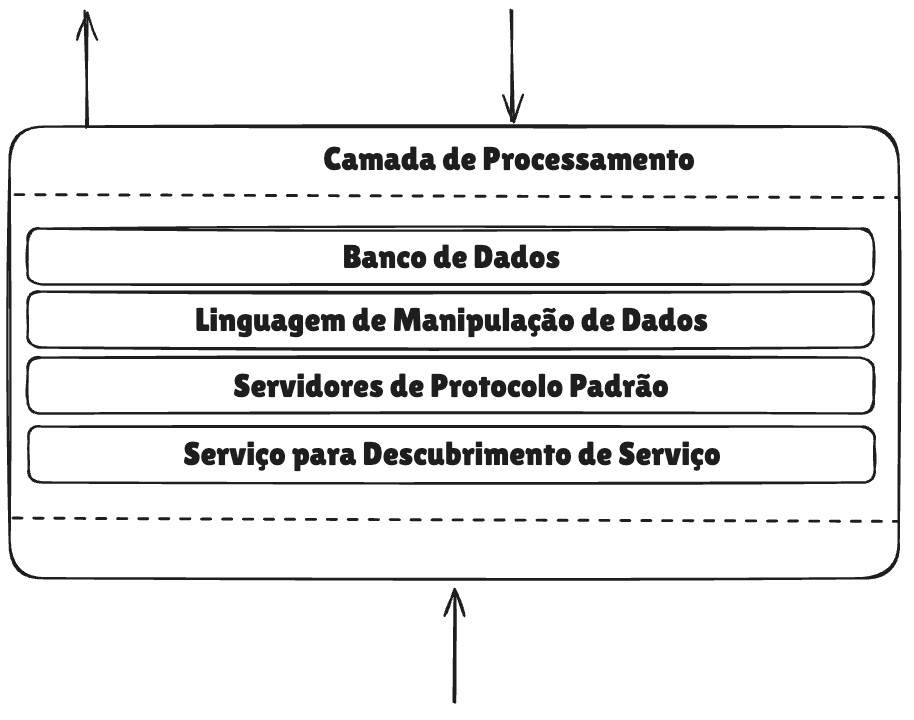
\includegraphics[width=0.7\linewidth]{images/camada_processamento.png}
    \end{center}
    \fonte{Do autor.}
\end{figure}

Na camada de serviços é executada a aplicação que implementa a lógica de pré-processamento dos dados. Utilizando a linguagem de consulta disponibilizada pela camada de processamento, essa camada obtém os dados necessários, executa o tratamento definido pela aplicação e devolve o resultado à camada de processamento, que, por sua vez, ajusta a saída para envio pela camada de protocolos.

% ----------------------------------------------------------
\subsection{Nó Agregador}
% ----------------------------------------------------------

O nó agregador atua como ponto central para receber os resultados pré-processados provenientes dos nós de névoa. Em vez de cada nó de névoa transmitir seus dados diretamente à nuvem, o agregador coleta e organiza essas informações, reunindo-as em um único conjunto consolidado.

Esse processo tem como efeito a redução da quantidade de requisições enviadas à nuvem, agrupando múltiplos envios menores em transmissões mais amplas e organizadas. Embora a redução de tráfego seja um dos resultados esperados, o principal papel do agregador é melhorar o fluxo de comunicação entre a camada de névoa e a nuvem, facilitando o controle, a rastreabilidade e a padronização dos dados enviados.

O nó agregador também pode executar transformações adicionais sobre os dados recebidos, como ajustes de formato, enriquecimento de metadados ou aplicação de funções específicas definidas pela aplicação. Após esse tratamento, os dados são preparados em lotes ou fluxos contínuos e encaminhados à nuvem de acordo com a política de envio configurada.

% ---

% ---
% 5 - Metodologia
% ---
% ----------------------------------------------------------
\chapter{Metodologia}
% ----------------------------------------------------------

\section{Tipo de Pesquisa}
Este trabalho caracteriza-se como uma pesquisa aplicada, de natureza tecnológica, com abordagem predominantemente qualitativa na fase de levantamento e definição de requisitos, e quantitativa na etapa de definição dos critérios de avaliação. O objetivo central é propor e modelar uma arquitetura modular de computação em névoa com suporte à comunicação entre múltiplas névoas.

\section{Procedimentos Metodológicos}

\subsection{Definição de Requisitos da Arquitetura}
A partir das lacunas identificadas na literatura (conforme discutido no Capítulo~\ref{cap:trabalhos_relacionados}), foram definidos requisitos funcionais e não funcionais, como:
\begin{itemize}
    \item Suporte à comunicação entre diferentes domínios de névoa;
    \item Capacidade de integração de dispositivos heterogêneos;
    \item Modularidade para implementação de múltiplos serviços;
    \item Balanceamento de carga e distribuição dinâmica de tarefas;
    \item Redução de latência e otimização do tráfego de rede.
\end{itemize}

\subsection{Modelagem da Arquitetura Modular}
A arquitetura proposta foi estruturada em três camadas principais:
\begin{itemize}
    \item \textbf{Nó Primário}: responsável pelo registro de dispositivos, balanceamento de carga entre nós locais e outros nós primários, e redirecionamento de tarefas.
    \item \textbf{Nós de Névoa}: responsáveis pela execução de serviços, pré-processamento e armazenamento temporário de dados.
    \item \textbf{Nó Agregador}: responsável por consolidar informações e preparar os dados para envio otimizado à nuvem.
\end{itemize}
Diagramas conceituais e funcionais foram elaborados para representar os componentes, fluxos de dados e protocolos de comunicação.

\subsection{Implementação em Ambiente Controlado}
A arquitetura foi implementada em ambiente local utilizando contêineres Docker, simulando medidores, nós de névoa e agregadores. Protocolos como HTTP e CoAP foram empregados para comunicação, e o gerenciamento de serviços foi desenvolvido em Python e Node.js. Essa configuração permitiu avaliar a viabilidade técnica e a escalabilidade horizontal da proposta.

\subsection{Definição dos Critérios de Avaliação}
Embora a validação experimental completa não tenha sido realizada no escopo deste trabalho, foram definidos critérios para avaliação futura:
\begin{itemize}
    \item Tempo de resposta (ms);
    \item Latência média (ms);
    \item Taxa de entrega de pacotes (\%);
    \item Escalabilidade (número de nós e dispositivos suportados).
\end{itemize}

\section{Ambiente e Ferramentas Utilizadas}
A implementação e simulação utilizaram os seguintes recursos:
\begin{itemize}
    \item Linguagens e frameworks: Python, Node.js;
    \item Infraestrutura de virtualização: Docker;
    \item Protocolos: HTTP, CoAP;
    \item Hardware: ambiente local com suporte a múltiplos contêineres e rede simulada;
    \item Ferramentas de modelagem: draw.io e ferramentas de diagramação compatíveis com \LaTeX.
\end{itemize}

\section{Fluxo Metodológico}
%A Figura~\ref{fig:fluxo_metodologia} apresenta o fluxo metodológico adotado, desde a definição dos requisitos até a implementação e definição dos critérios de avaliação.

%\begin{figure}[htb]
%	\caption{\label{fig:fluxo_metodologia}Fluxo metodológico do trabalho.}
%	\begin{center}
%		\includegraphics[width=0.9\linewidth]{images/fluxo_metodologia.png}
%	\end{center}
%	\fonte{Do autor.}
%\end{figure}

% ---

% ---
% 6 - Testes
% ---
%\phantompart
% ----------------------------------------------------------
\chapter{Testes}\label{cap:testes}
% ----------------------------------------------------------

Este capítulo descreve os procedimentos de teste adotados para avaliar a arquitetura proposta, abrangendo ambiente, cenários, métricas, coleta e análise dos dados.

% ----------------------------------------------------------
\section{Contextualização do Problema}
% ----------------------------------------------------------

Para avaliar a arquitetura proposta, foi adotado um cenário inspirado em aplicações de cidades inteligentes, com foco na gestão de recursos de água e energia. Nesse contexto, foram considerados medidores inteligentes que enviam dados de consumo para uma camada de névoa, onde ocorre o pré-processamento das informações antes de seu encaminhamento à nuvem.

Os dados utilizados para simulação foram obtidos a partir de conjuntos públicos, sendo um relacionado ao consumo residencial de energia elétrica \cite{uci_energy} e outro referente a medições de consumo de água \cite{greek_water}.

Antes da utilização nos testes, ambos os conjuntos de dados passaram por um processo de pré-processamento que incluiu a remoção de informações não essenciais e a agregação das medições em intervalos horários. Esse tratamento visou manter apenas os elementos relevantes para simular a operação contínua dos dispositivos, aproximando o comportamento dos dados ao fluxo esperado em um ambiente real de monitoramento urbano.

% ----------------------------------------------------------
\section{Ambiente de Testes}
% ----------------------------------------------------------

O ambiente de testes foi configurado para representar um cenário de cidade inteligente, no qual cada domínio de névoa corresponde a um bairro distinto. Cada névoa pode conter um nó primário, um nó agregador e um número variável de nós de névoa e dispositivos, de acordo com a demanda e o tipo de aplicação simulada.

A implantação e o gerenciamento desses componentes foram realizados por meio de uma interface web desenvolvida para este trabalho, que interage diretamente com o Docker para criar e controlar as instâncias. Essa interface permite selecionar o bairro (névoa) no qual os componentes serão implantados, definir o tipo de contêiner e a quantidade de instâncias, além de oferecer controle individual ou em grupo para iniciar, pausar, parar e visualizar logs.

A Figura~\ref{fig:container_manager} apresenta a tela de gerenciamento de contêineres para o bairro Canasvieiras. Nela, observa-se a criação de um nó de névoa e de um medidor de energia, ambos em execução. O painel agrupa as instâncias por tipo de componente, permitindo visualizar rapidamente seu estado e realizar ações sobre cada grupo ou instância individual.

\begin{figure}[htb]
    \caption{\label{fig:container_manager}Interface para gerenciamento de contêineres no ambiente de testes.}
    \begin{center}
        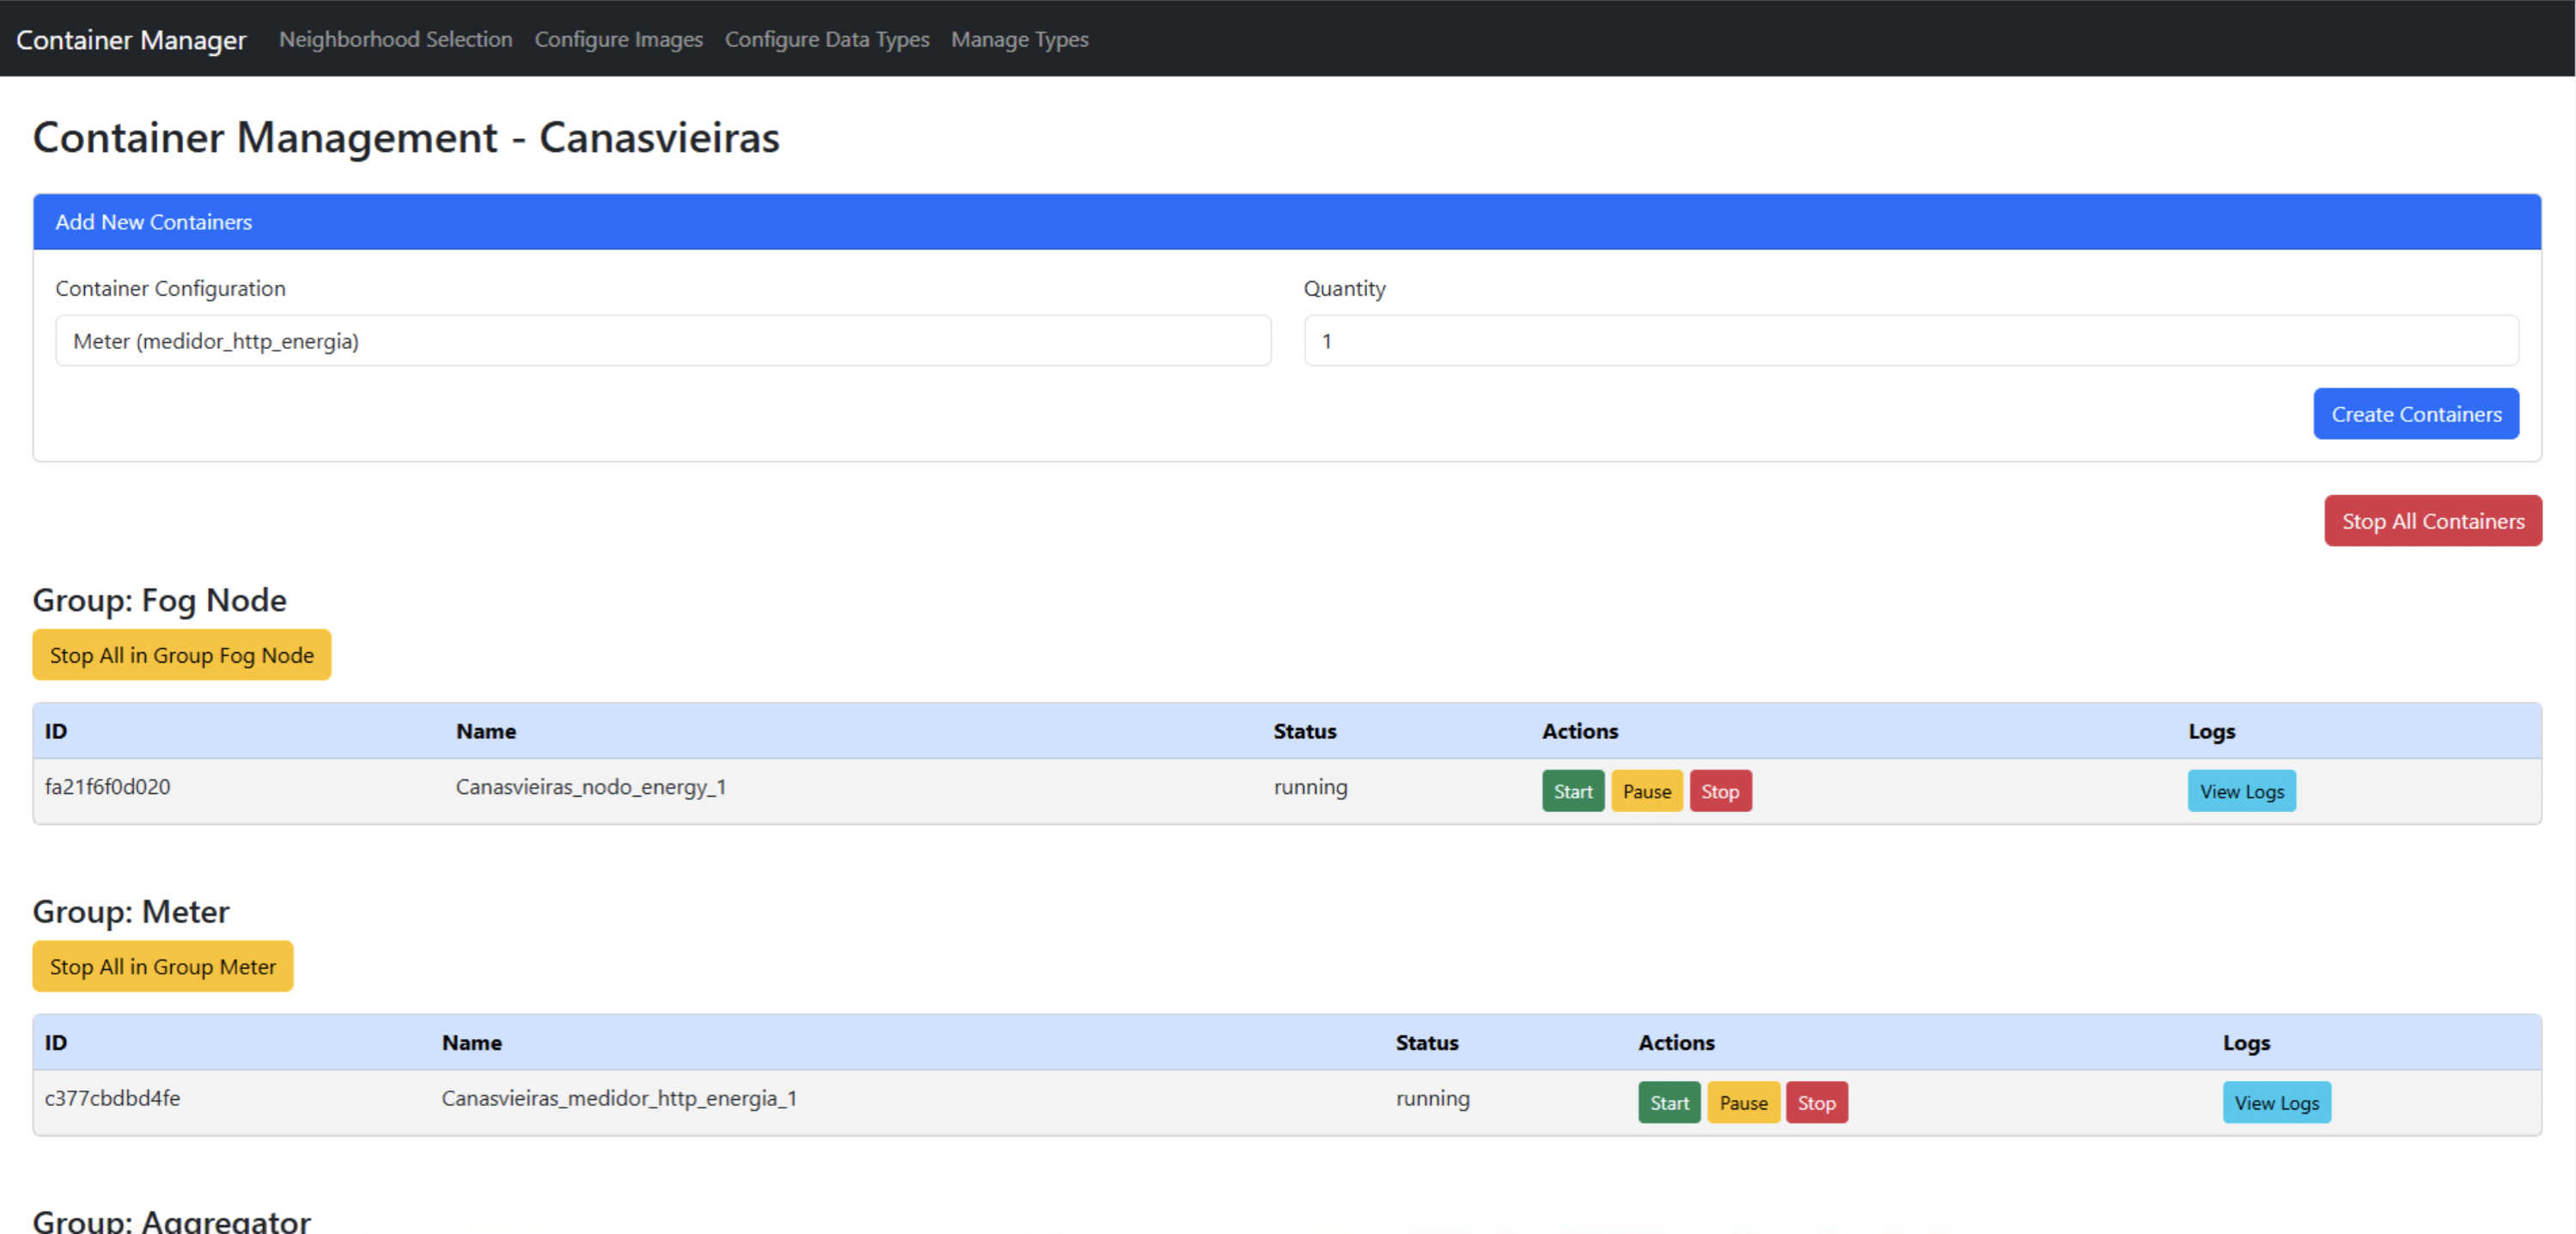
\includegraphics[width=1\linewidth]{images/container_manager.png}
    \end{center}
    \fonte{Do autor.}
\end{figure}

% ----------------------------------------------------------
\subsection{Tecnologias e Ambiente Físico}
% ----------------------------------------------------------

No ambiente de testes, todos os componentes da arquitetura foram implementados em \textit{Python}, com exceção do medidor compatível com o protocolo \textit{CoAP}, que foi desenvolvido em \textit{Node.js} devido à disponibilidade de bibliotecas específicas e otimização do fluxo de comunicação nesse protocolo.

Os experimentos foram executados em uma única máquina física, utilizada para hospedar os contêineres Docker que compõem cada instância de nó e dispositivo. A Tabela~\ref{tab:especificacoes_maquina} apresenta as especificações do equipamento utilizado.

\begin{table}[htb]
    \caption{\label{tab:especificacoes_maquina}Especificações da máquina utilizada nos testes.}
    \centering
    \begin{tabular}{ll}
        \hline
            \textbf{Componente} & \textbf{Especificação} \\
        \hline
            Processador & Intel Core i7-7700K @ 4.20GHz \\
            Memória RAM & 32 GB DDR4 \\
            Armazenamento & SSD 2 TB \\
            Sistema Operacional & Windows 11 \\
            Docker & v4.38.0 \\
        \hline
    \end{tabular}
    \fonte{Do autor.}
\end{table}

% ----------------------------------------------------------
\section{Protocolos}
% ----------------------------------------------------------

No ambiente de testes, o nó primário é responsável por receber dados utilizando diferentes protocolos, incluindo \textit{CoAP}, \textit{MQTT} e \textit{HTTP}. Independentemente do protocolo de origem, as mensagens são convertidas para \textit{HTTP} antes de serem encaminhadas aos nós de névoa, de forma a padronizar o tráfego interno.

Dentro de um nó de névoa, a comunicação entre a camada de protocolos e a camada de processamento ocorre por meio de \textit{WebSocket}, mantendo a conexão aberta para evitar o custo de abertura e fechamento contínuo de conexões. Essa abordagem reduz a sobrecarga e melhora o tempo de resposta.

A partir do nó de névoa, os dados já passam a ser organizados em estrutura \textit{CSV}, formada a partir das informações recebidas em \textit{JSON}. Essa etapa permite preparar os dados para compatibilidade com o formato aceito pela nuvem. A transmissão do nó de névoa para o nó agregador é realizada via \textit{SFTP}, garantindo a entrega confiável e preservando a integridade dos arquivos.

No nó agregador, os arquivos \textit{CSV} recebidos de diferentes nós de névoa são consolidados em um único arquivo antes de serem enviados para a camada de nuvem, também via \textit{SFTP}, para a zona de entrada (\textit{landing zone}) do \textit{HPCC Systems}.

Essa configuração busca compatibilidade entre os diferentes componentes, confiabilidade na entrega das mensagens e otimização do tráfego de rede.

% ----------------------------------------------------------
\section{Distribuição entre Névoas e Balanceamento de Carga}
% ----------------------------------------------------------

Nos experimentos, os \(120\) dispositivos foram distribuídos entre dois domínios de névoa distintos, representando diferentes regiões no cenário de cidade inteligente.  
A distribuição inicial foi a seguinte:

\begin{itemize}
    \item \textbf{Névoa A}: \(70\) dispositivos  
    (\(12\) medidores de energia via \textit{HTTP}, \(12\) via \textit{CoAP}, \(12\) via \textit{MQTT}, \(12\) medidores de água via \textit{HTTP}, \(12\) via \textit{CoAP}, \(10\) via \textit{MQTT}).
    \item \textbf{Névoa B}: \(50\) dispositivos  
    (\(8\) medidores de energia via \textit{HTTP}, \(8\) via \textit{CoAP}, \(8\) via \textit{MQTT}, \(8\) medidores de água via \textit{HTTP}, \(8\) via \textit{CoAP}, \(10\) via \textit{MQTT}).
\end{itemize}

Essa distribuição propositalmente desigual permitiu avaliar o comportamento do sistema sob condições de carga diferentes entre os domínios.  
Quando uma das névoas atingiu maior taxa de utilização, o mecanismo de balanceamento foi acionado: o nó primário da névoa mais carregada redirecionou parte das requisições para a outra, realizando a conversão para \textit{HTTP} antes do envio, independentemente do protocolo de origem (\textit{HTTP}, \textit{CoAP} ou \textit{MQTT}).

Nos testes, foram simulados dois dias de operação (\(48\ \text{horas}\)), com cada dispositivo enviando leituras periódicas agregadas em janela horária de consumo.

No nó agregador, as medições de cada domínio de névoa foram consolidadas em um único arquivo por dia e transmitidas para o \textit{HPCC Systems} ao final de cada dia, sem que nenhum contêiner apresentasse falhas durante a execução.

% ----------------------------------------------------------
\section{GraphQL}
% ----------------------------------------------------------

Nos nós de névoa, a comunicação entre a camada de serviços e a camada de processamento é realizada utilizando \textit{GraphQL} como linguagem de consulta de dados. Essa abordagem permite que a aplicação especifique exatamente quais campos e registros deseja receber, evitando transferências desnecessárias e reduzindo a sobrecarga de processamento.  

O \textit{GraphQL} possibilita ainda a consulta a múltiplas fontes de dados de forma unificada, agregando resultados distintos em uma única resposta. Nos testes realizados, o armazenamento local temporário nos nós de névoa foi implementado com \textit{MongoDB}, escolhido por sua flexibilidade para lidar com dados em formato \texttt{JSON} e pela capacidade de inserir registros heterogêneos sem a exigência de um esquema fixo.  

Com essa integração, a camada de serviços consegue solicitar à camada de processamento apenas as informações estritamente necessárias para o pré-processamento, recebendo uma resposta já filtrada e adaptada ao contexto da aplicação. Isso mantém a arquitetura modular, otimiza o fluxo de dados interno e garante maior agilidade na execução das tarefas.

% ----------------------------------------------------------
\section{HPCC Systems na Camada de Nuvem}
% ----------------------------------------------------------

Na fase de testes, os dados consolidados pelos nós agregadores foram enviados para a camada de nuvem, implementada com o \textit{HPCC Systems}. Os arquivos recebidos, no formato \texttt{.csv} suportado pela plataforma, resultam da união dos pré-processamentos realizados nos diferentes nós de névoa, reunidos pelo nó agregador antes da transmissão.  

Esses arquivos foram disponibilizados na zona de entrada da plataforma (\textit{landing zone}), onde ficaram prontos para processamento e consultas.  

A Figura~\ref{fig:hpcc_landing_zone} apresenta o ambiente \textit{ECL Watch}, mostrando os arquivos agregados de consumo de energia, já no formato consolidado por data, prontos para serem tratados ou analisados conforme as necessidades da aplicação.

\begin{figure}[htb]
    \caption{\label{fig:hpcc_landing_zone}Arquivos consolidados na \textit{landing zone} do HPCC Systems.}
    \begin{center}
        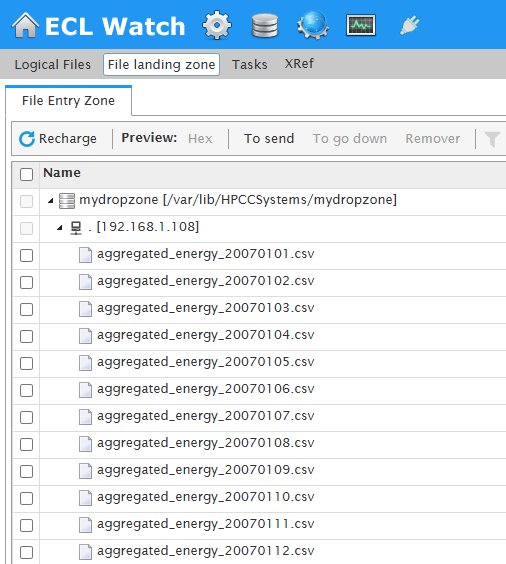
\includegraphics[width=0.7\linewidth]{images/hpcc_landing_zone.png}
    \end{center}
    \fonte{Do autor.}
\end{figure}


% ---
% 7 - Resultados
% ---
%\phantompart
% ----------------------------------------------------------
\chapter{Resultados}\label{cap:resultados}
% ----------------------------------------------------------

Esta seção apresenta as métricas obtidas nos testes da arquitetura proposta.  
Para cada métrica, é mostrado o cálculo realizado com base nos valores coletados e, em seguida, um parágrafo explicando seu significado e comentando o valor obtido.

% ----------------------------------------------------------
\section{Valores Medidos}
% ----------------------------------------------------------

Os valores apresentados nas Tabelas~\ref{tab:latencias} e~\ref{tab:memoria} foram obtidos a partir de \textit{timestamps} registrados nos pontos de entrada e saída de cada componente, bem como de medições de consumo de memória realizadas durante o envio de mensagens.  

A Tabela~\ref{tab:latencias} mostra as latências médias unidirecionais para cada segmento do fluxo, abrangendo desde a recepção inicial no \textit{Load Balancer} até o envio final ao HPCC Systems, enquanto a Tabela~\ref{tab:memoria} apresenta o consumo médio de memória por componente.  

Observa-se que o maior tempo de transmissão ocorre no trajeto entre o Agregador e o HPCC Systems, indicando que esta etapa concentra a maior parte da latência no fluxo de dados. Em relação ao uso de memória, verifica-se que os nós de névoa demandam mais recursos, devido às tarefas de pré-processamento e armazenamento temporário, enquanto os componentes de controle, como o \textit{Load Balancer} e o Agregador, apresentam consumo significativamente menor.

\begin{table}[htb]
    \caption{\label{tab:latencias}Latências médias unidirecionais medidas}
    \centering
    \begin{tabular}{|l|c|}
        \hline
            \textbf{Caminho} & \textbf{Latência (ms)} \\
        \hline
            Medidor $\rightarrow$ Load Balancer & 4,6 \\
            Load Balancer $\rightarrow$ Nó de Névoa & 2,0 \\
            Nó de Névoa $\rightarrow$ Agregador & 2,4 \\
            Agregador $\rightarrow$ HPCC Systems & 6,6 \\
        \hline
    \end{tabular}
    \fonte{Do autor.}
\end{table}

\begin{table}[htb]
    \caption{\label{tab:memoria}Consumo médio de memória por componente}
    \centering
    \begin{tabular}{|l|c|}
        \hline
            \textbf{Componente} & \textbf{Memória (MiB)} \\
        \hline
            Load Balancer & 37,37 \\
            Agregador & 40,14 \\
            Nó de Névoa (Energia) & 276,60 \\
            Simulador de Medidor HTTP & 19,97 \\
        \hline
    \end{tabular}
    \fonte{Do autor.}
\end{table}

% ----------------------------------------------------------
\section{Latência ponta a ponta}
% ----------------------------------------------------------

\[
L_t = L_{ml} + L_{ln} + L_{na} + L_{ah}
\]

Onde:  
\begin{itemize}
    \item \(L_{ml}\) = latência do Medidor → Load Balancer = \(4{,}6\ \text{ms}\)
    \item \(L_{ln}\) = latência do Load Balancer → Nó de Névoa = \(2{,}0\ \text{ms}\)
    \item \(L_{na}\) = latência do Nó de Névoa → Agregador = \(2{,}4\ \text{ms}\)
    \item \(L_{ah}\) = latência do Agregador → HPCC Systems = \(6{,}6\ \text{ms}\)
\end{itemize}

\[
L_t = 4{,}6 + 2{,}0 + 2{,}4 + 6{,}6 = 15{,}6 \ \text{ms}
\]

O cálculo considera a soma das latências médias unidirecionais medidas para cada segmento do fluxo de transmissão.

% ----------------------------------------------------------
\section{Throughput}
% ----------------------------------------------------------

\[
\text{Throughput} = \frac{M_p}{T}
\]

Onde:  
\begin{itemize}
    \item \(N_d\) = número de dispositivos = \(120\)
    \item \(F_m\) = frequência de envio de mensagens (mensagens por hora) = \(1\)
    \item \(T\) = duração total do experimento = \(48\ \text{h}\)
    \item \(M_p\) = total de mensagens processadas = \(5{,}760\)
\end{itemize}

\[
\text{Throughput} = \frac{5{,}760}{48} = 120\ \text{msgs/h}
\]

O cálculo considera a quantidade de mensagens processadas dividida pelo tempo total do experimento, resultando no número médio de mensagens processadas por hora.

% ----------------------------------------------------------
\section{Taxa de entrega}
% ----------------------------------------------------------

\[
M_e = N_d \times F_m \times T = 120 \times 1 \times 48 = 5{,}760
\]

\[
\text{Taxa de entrega} = \frac{M_r}{M_e} \times 100
\]

Onde:  
\begin{itemize}
    \item \(M_r\) = quantidade total de mensagens recebidas = \(5{,}760\)
    \item \(M_e\) = quantidade total de mensagens esperadas = \(5{,}760\)
\end{itemize}

\[
\text{Taxa de entrega} = \frac{5{,}760}{5{,}760} \times 100 = 100\%
\]

O cálculo considera a razão entre a quantidade de mensagens recebidas e o total esperado no período do experimento.

% ----------------------------------------------------------
\section{Fator de agregação}
% ----------------------------------------------------------

\[
\rho = \frac{M_r}{M_n}
\]

Onde:  
\begin{itemize}
    \item \(M_r\) = mensagens recebidas pelo agregador em dois dias = \(2 \times 2880 = 5760\)
    \item \(M_n\) = mensagens enviadas à nuvem pelo agregador no mesmo período = \(2\)
\end{itemize}

\[
\rho = \frac{5760}{2} = 2880
\]

O cálculo considera a razão entre a quantidade de mensagens recebidas pelo agregador e o número de mensagens enviadas à nuvem em um mesmo intervalo de tempo.

% ----------------------------------------------------------
\section{Redução de requisições à nuvem}
% ----------------------------------------------------------

\[
\text{Redução}(\%) = \frac{(N_d \times M_d \times 2) - M_a}{N_d \times M_d \times 2} \times 100
\]

Onde:  
\begin{itemize}
    \item \(N_d\) = número de dispositivos = \(120\)
    \item \(M_d\) = mensagens enviadas por dispositivo/dia = \(24\)
    \item \(M_a\) = mensagens enviadas via agregador no total de dois dias = \(2\)
\end{itemize}

\[
\text{Redução}(\%) = \frac{(120 \times 24 \times 2) - 2}{120 \times 24 \times 2} \times 100
= \frac{5760 - 2}{5760} \times 100
\approx 99{,}97\%
\]

O cálculo considera a quantidade total de mensagens enviadas diretamente pelos dispositivos no período de dois dias, comparada ao número de mensagens transmitidas via agregador no mesmo período.


% ---
% 8 - Conclusão
% ---
%\phantompart
% ----------------------------------------------------------
\chapter{Conclusão}\label{cap:conclusao}
% ----------------------------------------------------------

Este trabalho apresentou o desenvolvimento e a avaliação de uma arquitetura modular para ambientes de computação em névoa, com suporte à comunicação direta entre domínios distintos e integração entre dispositivos de borda, nós de névoa e a nuvem, tomando como referência o modelo proposto pelo OpenFog Consortium~\cite{openfog2018}. A solução foi projetada considerando os principais pilares dessa arquitetura no contexto de cidades inteligentes, buscando atender às diretrizes de escalabilidade, abertura, autonomia, programabilidade e hierarquia.

A escalabilidade foi contemplada na forma como a infraestrutura pode ser expandida sem reconfigurações complexas, permitindo a adição de novos nós ou dispositivos de maneira transparente. A abertura esteve presente no suporte a diferentes protocolos de comunicação, favorecendo a interoperabilidade entre sistemas heterogêneos. A autonomia foi explorada por meio do balanceamento de carga dinâmico e distribuído entre domínios, dispensando a necessidade de um ponto central de orquestração. A programabilidade se refletiu na flexibilidade para ajustar o comportamento do balanceador e dos nós de névoa de acordo com as necessidades do cenário de uso. Já a hierarquia esteve evidente na organização em camadas, interligando dispositivos de borda, névoa e nuvem de forma estruturada e modular.

Os resultados obtidos indicam que a combinação de abstração de protocolos, balanceamento dinâmico de carga e alto fator de agregação contribuiu para reduzir o volume de requisições à nuvem e melhorar a utilização dos recursos, mantendo tempos de resposta compatíveis com aplicações sensíveis à latência.

Na comparação com trabalhos como o EXEGESIS~\cite{exegesis2021}, que permite a substituição de serviços em ambiente de execução por meio da reconstrução do contêiner, a arquitetura proposta requer a interrupção para a troca de serviços. No entanto, a separação entre a camada de aplicação e as demais possibilita interromper apenas a aplicação, realizar os ajustes necessários e retomá-la sem modificar a lógica de comunicação. Durante esse processo, a camada de protocolos permanece ativa, continuando a receber dados, processá-los e armazená-los temporariamente, o que contribui para reduzir perdas e facilitar a retomada do serviço. Essa característica pode simplificar a manutenção e a adaptação a novos requisitos, minimizando o impacto de mudanças, ainda que a substituição implique uma breve indisponibilidade. Além disso, o encaminhamento distribuído entre névoas permite o tráfego direto de dados entre domínios, evitando a necessidade de um ponto único de orquestração.

Como contribuição, o trabalho demonstrou a viabilidade de integrar múltiplos protocolos e distribuir cargas entre diferentes domínios de névoa sem comprometer o desempenho. Para trabalhos futuros, sugere-se a adoção de mecanismos de autenticação e criptografia ponta a ponta, a implementação de estratégias de recuperação automática em caso de falhas e a aplicação da arquitetura em outros domínios, como saúde conectada e transporte inteligente, considerando diferentes perfis de tráfego e demanda.


% ----------------------------------------------------------
% ELEMENTOS PÓS-TEXTUAIS
% ----------------------------------------------------------
%\postextual
% ----------------------------------------------------------

% ----------------------------------------------------------
% Referências bibliográficas
% ----------------------------------------------------------
\begingroup
    \SingleSpacing\printbibliography
\endgroup

% ----------------------------------------------------------
% Glossário
% ----------------------------------------------------------
%
% Consulte o manual da classe abntex2 para orientações sobre o glossário.
%
%\glossary

% ----------------------------------------------------------
% Apêndices
% ----------------------------------------------------------

% ---
% Inicia os apêndices
% ---
%\begin{apendicesenv}
%	\partapendices* 
%	\counterwithin{figure}{chapter}
%	% ----------------------------------------------------------
\chapter{Descrição 1}
% ----------------------------------------------------------

Textos elaborados pelo autor, a fim de completar a sua argumentação. Deve ser precedido da palavra APÊNDICE, identificada por letras maiúsculas consecutivas, travessão e pelo respectivo título. Utilizam-se letras maiúsculas dobradas quando esgotadas as letras do alfabeto. 

%\end{apendicesenv}
% ---


% ----------------------------------------------------------
% Anexos
% ----------------------------------------------------------

% ---
% Inicia os anexos
% ---
%\begin{anexosenv}
%	\partanexos*
%	% ----------------------------------------------------------
\chapter{Descrição 2}
% ----------------------------------------------------------

São documentos não elaborados pelo autor que servem como fundamentação (mapas, leis, estatutos). Deve ser precedido da palavra ANEXO, identificada por letras maiúsculas consecutivas, travessão e pelo respectivo título. Utilizam-se letras maiúsculas dobradas quando esgotadas as letras do alfabeto. 

%\end{anexosenv}

%---------------------------------------------------------------------
% INDICE REMISSIVO
%---------------------------------------------------------------------
%\phantompart
%\printindex
%---------------------------------------------------------------------

\end{document}
